\documentclass[11pt]{article}
\usepackage[margin=1in]{geometry}
\usepackage{parskip}
\renewcommand{\baselinestretch}{1.35}
\usepackage[slovak]{babel}
\usepackage{fancyhdr}
\usepackage{enumitem}
\usepackage{gensymb}
\usepackage[utf8]{inputenc}
\usepackage{amsmath, amssymb, amsfonts}
\usepackage{graphicx, caption}
\graphicspath{ {./images/} }
\usepackage{algorithm}
\usepackage{algpseudocode}


\title{\textbf{Úkol č. 2: Generalizácia budov}}
\author{Hugo Majer, Júlia Šušková}


\begin{document}

%%%%%%%%%%%%%%%%%% TITUL %%%%%%%%%%%%%%%%%%%%%%%%
\pagenumbering{gobble}
\maketitle

\newpage
\pagenumbering{arabic}
%%%%%%%%%%%%%%%%%%%%%%%%%%%%% ZADANIE %%%%%%%%%%%%%%%%%%%%%%%%%%%%%%%
\section{Zadanie}
\textbf{Úloha č. 2: Generalizace budov}

\textit{Vstup: množina budov $B = \{Bi\}$, budova $Bi = \{P_{i,j}\}$}\\
\textit{Výstup: $G(Bi)$.}

Ze souboru načtěte vstupní data představová lomovými body budov. Pro tyto účely použijte vhodnou datovou
sadu, např. ZABAGED.

Pro každou budovu určete její hlavní směry metodami \textit{Minimum Area Enclosing Rectangle}, \textit{Wall Average}.

U první metody použijte některý z algoritmů pro konstrukci konvexní obálky. Budovu nahraďte obdélníkem se
středem v jejím těžišti orientovaným v obou hlavních směrech, jeho plocha bude stejná jako plocha budovy. Výsledky generalizace vhodně vizualizujte.

Odhadněte efektivitu obou metod, vzájemně je porovnejte a zhodnoťte. Pokuste se identifikovat, pro které tvary budov dávají metody nevhodné výsledky, a pro které naopak poskytují vhodnou aproximaci.

\newpage
\section{Údaje o bonusových úlohách}
Boli riešené nasledujúce bonusové úlohy:

\textit{Generalizace budov metodou Longest Edge. (+5b)\\
Generalizace budov metodou Weighted Bisector. (+8b)\\
Implementace další metody konstrukce konvexní obálky (Graham Scan). (+5b)\\
Ošetření singulárního případu při generování konvexní obálky. (+2b)}

\setlength{\parindent}{1cm}
\newpage
%%%%%%%%%%%%%%%%%%%%%%% Generalizacia budov %%%%%%%%%%%%%%%%%%%%%%%%%%%%%%%

\section{Generalizácia budov} \label{gb}
Kartografická generalizácia je procedúra redukcie reality, ktorou sa kartografovia zaoberajú od nepamäti. Pri tvorbe máp častokrát dochádza k situácií, kedy do mapy nie je možné úplne exaktne a geometricky presne vyjadriť obrazy objektov, procesov a ich vzťahy. Vtedy je nutné vytvoriť zjednodušené a zovšeobecnené obrazy týchto elementov, inými slovami potlačiť nepodstatné a ponechať len určité charakteristické črty daných elementov. Podstatné a nepodstatné prvky definuje napríklad merítko mapy a jej účel. Postup a spôsob generalizácie ale nie je unifikovaný a výsledok je vždy určitý kompromis (Droppová, 2011).

Automatizovanou generalizáciou sa kartografovia zaoberajú od 60. rokov minulého storočia. Na prelome tisícročí bolo vyvinutých mnoho geometrických algoritmov a ako výsledok vzniklo aj mnoho generalizačných algoritmov bodových, líniových a plošných prvkov mapy. Tieto algoritmy vykonávajú geometrickú transformáciu (Li et al., 2004).

Predmetom tejto práce je generalizácia budov. Tá môže zahrňovať ich výber, agregáciu, ale hlavne zjednodušenie obrysu budovy, hlavne za účelom zlepšiť vizuálnu kvalitu mapy. Počas tohto procesu musia byť zachované typické vlastnosti danej budovy (Sester, 2018). Tá je vo všeobecnosti popísaná pozíciou, tvarom, veľkosťou a orientáciou, pričom práve orientácia budovy bude skúmanou vlastnosťou v rámci tejto práce (Duchene et al., 2003). 

Obrazom budovy v mape je polygón, u ktorého je pomerne obtiažné určiť orientáciu. U určitých tvarov budov je určenie orientácie celkom bezproblémové a priamočiare, ale takisto existujú tvary budov u ktorých určenie orientácie nie je možné. Práve z tohto dôvodu je ťažké definovať, čo vôbec orientácia budovy predstavuje (Duchene et al., 2003).\newline
Orientácia budovy môže byť predstavovaná tzv. hlavnými smermi budovy, pomocou ktorých môžeme popísať jej natočenie voči ostatným prvkom mapy. Tento vzťah voči iným prvkom musí byť pri generalizácií budovy zachovaný, tj. totožný ako pred generalizáciou danej budovy. 

Na určenie hlavných smerov budovy existuje viacero algoritmov, uveďme napr. \textit{Minimum Area Enclosing Rectangle}, \textit{Wall Average}, \textit{Longest Edge} a \textit{Weighted Bisector}.

\newpage
\section{Minimum Area Enclosing Rectangle} \label{maer}
Uvažujme, že vstupom do procesu generalizácie budovy je polygón $B$ tvorený lomovými bodmi $\{P_i\}$, pričom $P_i = [x_i, y_i]$. Hrany polygónu $B$ nie sú rovnobežné s osami $X$ a $Y$, ale sú voči ním orientované pod nejakým uhlom $\sigma$, ktorý musí byť detegovaný. Pre túto úlohu sa najčastejšie volí algoritmus \textit{Minimum Area Enclosing Rectangle}, ktorý konštruuje obdĺžnik tak, aby obklopoval všetky lomové body budovy a aby jeho plocha bola minimálna. Tento obdĺžnik sa nazýva \textit{Minimum Bounding Box}. Uhol $\sigma$ je potom formovaný osou $X$ a dlhšou stranou opisovaného obdĺžnika (Bayer, 2008). Prvý krok tohto algoritmu avšak pozostáva z tvorby konvexnej obálky, pre ktorú boli zvolené algoritmmi \textit{Jarvis Scan} a \textit{Graham Scan}.

\subsection{Jarvis Scan} \label{js}
Pod pojmom konvexná obálka $H$ rozumieme najmenší možný konvexný polygón, ktorý obklopuje vstupnú množinu bodov tak, že každý bod leží v jeho vnútri alebo na jeho obvode (tvorí hranu polygónu). 

Na vstupe do \textit{Jarvis Scan} máme množinu bodov $\{P_i\}$. Dva posledné body tvorenej  konvexnej obálky $H$ označujeme ako $P_{j-1}$ a $P_j$. Bod $P_{j+1}$ predstavuje aktuálne pridávaný bod do $H$. Ten musí maximalizovať uhol $\omega(P_{j-1}, P_j, P_i)$, pričom daný bod $P_i \notin H$:
\begin{equation*}
P_{j+1} = max \: \omega(P_{j-1}, P_j, P_i) 
\end{equation*}
\noindent Samotné uhly $\omega(P_{j-1}, P_j, P_i)$ spočítame pomocou známeho vzorca pre odchýlku dvoch vektorov $\vec{u}$ a $\vec{v}$, pričom $\vec{u}$ je smerový vektor priamky $\overleftrightarrow{P_{j-1}P_j}$ a $\vec{v}$ smerový vektor priamky $\overleftrightarrow{P_jP_i}$:
\begin{equation*}
\cos\omega=\frac{\vec{u}\vec{v}}{\lVert\vec{u}\rVert\lVert\vec{v}\rVert}
\end{equation*}

\textit{Jarvis Scan} je považovaný za jeden z prvých moderných algoritmov, je ľahko implementovateľný a formálne pseudokódom sa dá zapísať nasledovne:
\begin{algorithm}
    \caption {\textit{Jarvis Scan}}
    \begin{algorithmic}[1]
        \State Nájdenie bodu $P_{min}$ s minimálnou $y$ súradnicou, $P_{min}$ = min$(y_i)$.
        \State Pridaj bod $P_{min}$ do tvorenej konvexnej obálky $H$: $P_{min} \in H$.
        \State Inicializuj posledné dva body $H$: $P_{j-1} = [-\infty,$ min$(y_i)]$, $P_j = P_{min}$.
        \State Inicializuj pridávaný bod do $H$: $P_{j+1} = P_{j-1}$.
        \State Pokým $P_{j+1} \neq P_{min}$:
        \State \indent Pre každý vstupný bod $P_i$:
        \State \indent \indent Spočítaj uhol $\omega(P_{j-1}, P_j, P_i)$.
        \State \indent Nastav $P_{j+1} =$ max $\omega(P_{j-1}, P_j, P_i)$.
        \State \indent Pridaj $P_{j+1}$ do konvexnej obálky $H$: $P_{j+1} \in H$.
        \State \indent Aktualizuj posledné dva body $H$: $P_{j-1}$ = $P_j$, $P_j = P_i$.
    \end{algorithmic}
\end{algorithm}
\newpage
\subsection{Graham Scan} \label{gs}
Algoritmus \textit{Graham Scan} je veľmi efektívny algoritmus, ktorý je založený na kritériu ľavotočivosti. Pozostáva z tvorby \textit{star-shaped} polygónu z bodu $P_{min}$, ktorý predstavuje bod s minimálnou \linebreak súradnicou $y$. Jeho vrcholy sú zoradené podľa uhlu $\omega(X, P_{min}, P_i)$. Pri uhle $\omega$ sa môže vyskytnúť situácia, kedy viacero bodov má rovnaký uhol $\omega$. V takomto prípade sa ponechá len ten bod, ktorý je najvzdialenejší od bodu $P_{min}$.

Ľavotočivosť zabezpečujeme Half-Plane testom. Vždy z posledných dvoch bodov konvexnej obálky, označme ich $P_t = [x_t, y_t]$ a $P_{t-1} = [x_{t-1}, y_{t-1}]$, sa vytvorí priamka $p$ voči ktorej určujeme pozíciu nasledujúceho bodu konvexnej obálky, označme ho $P_j = [x_j, y_j]$.\newline
\textit{Poznámka}: Posledné, resp. prvé dva body konvexnej obálky na začiatku predstavuje bod $P_{min}$ a bod $P_i$, v ktorom je uhol $\omega(X, P_{min}, P_i)$ minimálny.
\begin{align}
    \nonumber&\vec{u}=(x_t - x_{t-1}, y_t - y_{t-1})\\
    \nonumber&\vec{v}=(x_j - x_t, y_j - y_t)
\end{align}
Za pomoci vektorového súčinu smerových vektorov $\vec{u}$ a $\vec{v}$ zapísaného maticovo a pomocou znamienka determinantu určíme, v ktorej polrovine voči priamke $p(P_t, P_{t-1})$ sa bod $P_j$ nachádza:
\begin{equation*}
t=\begin{vmatrix} u_x & u_y \\ v_x & v_y  \end{vmatrix}=u_x*v_y-v_x*u_y \Rightarrow
\begin{cases}
    t>0, \quad P_j(p) \in \sigma_l \\
    t=0, \quad P_j(p) \in p\\
    t<0, \quad P_j(p)  \in \sigma_r
\end{cases}
\end{equation*}
Ak bod $P_j \in \sigma_l$ alebo $P_j \in p$ (kolinearita), tak bude tvoriť konvexnú obálku $H$, tj. $P_j \in H$. Ak bod $P_j \in \sigma_r$, tak posledný bod konvexnej obálky $P_t$ bude z nej vyradený, tým pádom poslednými dvoma bodmi $H$ bude $P_{t-1}$ a $P_{t-2}$.
\newpage
\begin{algorithm}
    \caption {\textit{Graham Scan}}
    \begin{algorithmic}[1]
        \State Nájdenie bodu $P_{min}$ s minimálnou $y$ súradnicou, $P_{min}$ = min$(y_i)$.
        \State Pre každý bod $P_i$:
        \State \indent Spočítaj uhol $\omega(X, P_{min}, P_i)$.
        %\State Spoj $P_{min}$ s každým bodom a spočítaj uhol spojnice a osi X.
        \State Zoraď body $P_i$ podľa uhlu $\omega$ od najmenšieho po najväčší, index $j$ odpovedá zoradenému poradiu, $n$ odpovedá počtu bodov.
        \State Ak existujú body s rovnakým uhlom $\omega$, ponechaj len ten najvzdialenejší od $P_{min}$.
        \State Inicializuj prvé dva body konvexnej obálky: $P_{min}$, a bod $P_i =$ min $\omega(X, P_{min}, P_i)$, tj. bod s indexom $j = 0$.
        \State Inicializuj $j = 1$.
        \State Pokým $j < n$:
        \State \indent Ak $P_j(p) \in \sigma_l$ voči priamke $p(P_t, P_{t-1})$ ($P_t, P_{t-1}$ sú posledné dva body $H$).
        \State \indent \indent $P_j \in H$.
        \State \indent \indent Aktualizuj posledné dva body konvexnej obálky $H$: $P_j = P_t$, $P_{t-1} = P_t$
        \State \indent \indent Aktualizuj $j = j + 1$.
        \State \indent Ak je $P_j(p) \in \sigma_r$ voči priamke $p(P_t, P_{t-1})$:
        \State \indent \indent Posledný bod konvexnej obálky $P_t$ vyraď z konvexnej obálky $H$.
        \State \indent \indent Aktualizuj posledné dva body konvexnej obálky $H$: $P_t = P_{t-1}$, $P_{t-1} = P_{t-2}$
    \end{algorithmic}
\end{algorithm}
\subsection{Minimum Bounding Box}\label{mbb}
Po vytvorení konvexnej obálky $H$ môžeme pristúpiť k tvorbe \textit{Minimum Bounding Box}, tj. obdĺžnik, ktorý obklopuje všetky lomové body budovy a jeho plocha je minimálna. Dochádza ku opakovanej rotácií množiny vstupných lomových bodov $\{P_i\}$ o uhol $-\sigma$, ktorý je predstavovaný zápornou hodnotou smernice $\sigma$ určitej hrany konvexnej obálky $H$. Dochádza vlastne k tomu, že konvexnú obálku "postavíme" na danú hranu. \newline Stanovme, že hrana konvexnej obálky $H$ je tvorená bodmi $C_i = [x_i, y_i]$ a $C_{i+1} = [x_{i+1}, y_{i+1}]$. Smernicu hrany konvexnej obálky $H$ spočítame nasledovne:
\begin{align}
    \nonumber&\Delta x = x_{i+1} - x_i\\
    \nonumber&\Delta y = y_{i+1} - y_i\\\bigskip
    \nonumber&\tan \sigma = \frac{\Delta y}{\Delta x}
\end{align}
Vstupné lomové body, resp. konvexnú obálku rotujeme o $-\sigma$ za pomoci matice rotácie:\newline
\begin{equation*}
    \begin{pmatrix}
        \cos (-\sigma) & - \sin (-\sigma)\\
        \sin (-\sigma) & \cos (-\sigma)
    \end{pmatrix}
    \begin{pmatrix}
        x\\
        y
    \end{pmatrix}
    =
    \begin{pmatrix}
        x_r\\
        y_r
    \end{pmatrix}
\end{equation*}

\indent V takejto polohe je konštruovaný \textit{Minimum Bounding Box} konvexnej obálky.
%množiny vstupných lomových bodov $\{P_i\}$, $P_i = [x_i, y_i]$. 
V prvom rade musíme nájsť vrcholy tohto obdĺžniku, ktoré sú tvorené pomocou horných a spodných extrémov súradníc $x_i$ a $y_i$. Pre vytvorený \textit{Minimum Bounding Box} spočítame plochu $S$, spôsobom klasickým pre obdĺžnik. Takto vytvorený \textit{Minimum Bounding Box} následne otočíme naspäť do pôvodnej polohy a to za pomoci uvedenej matice rotácie (uhol otočenia je ale $\sigma$) a samozrejme platí, že otočením sa plocha $S$ nezmení.
\noindent Výsledným \textit{Minimum Bounding Box} po iterácií cez každú hranu konvexnej obálky je ten, ktorý má najmenšiu plochu $S$. Uhol, resp. smernicu hrany konvexnej obálky, v ktorej bol skonštruovaný označme $\sigma_{min}$.

Výsledný \textit{Minimum Bounding Box} je nutné ešte upraviť tak, aby mal plochu $S$ totožnú s plochou budovy $S_b$, ktorú aproximuje. Plochu budovy $S_b$, ktorá má tvar polygónu spočítame pomocou L'Huillierovho vzorca nasledovne:
\begin{equation*}
S_b = \sum_{i=1}^{n} \frac{x_i(y_{i+1}-y_{i-1})}{2}
\end{equation*}
Následne spočítame pomer $k$, medzi plochou budovy $S_b$ a plochou \textit{Minimum Bounding Box} $S$:
\begin{equation*}
k = \frac{S_b}{S} 
\end{equation*}
Nech vrcholy \textit{Minimum Bounding Box} tvorí štvorprvková množina $\{V_i\}$. Za využitia ťažiska \textit{Minimum Bounding Box} $T$ spočítame smerové vektory jeho uhlopriečok:
\begin{align}
    \nonumber &\vec{u_1} = V_1 - T\\
    \nonumber &\vec{u_2} = V_2 - T\\
    \nonumber &\vec{u_3} = V_3 - T\\
    \nonumber &\vec{u_4} = V_4 - T
\end{align}
Nové vrcholy \textit{Minimum Bounding Box} $\{V'_i\}$ vypočítame ako:
\begin{align}
    \centering
    \nonumber &V'_1 = T + \sqrt{k} \vec{u_1}\\
    \nonumber &V'_2 = T + \sqrt{k} \vec{u_2}\\
    \nonumber &V'_3 = T + \sqrt{k} \vec{u_3}\\
    \nonumber &V'_4 = T + \sqrt{k} \vec{u_4}
\end{align}
\textit{Minimum Bounding Box} tvorený vrcholmi $\{V'_i\}$ ná rovnakú plochu $S$ ako plocha budovy $S_b$.

Vo finále aproximáciou budovy je obdĺžnik, ktorý má rovnakú plochu $S$ ako budova a jeho orientácia (natočenie) je totožná s uhlom $\sigma_{min}$, tj. uhlom, v ktorom bol nájdený optimálny \textit{Minimum Bounding Box}, tj. taký, ktorý mal najmenšiu plochu $S$.     
\newpage
\noindent Pseudokód algoritmu \textit{Minimum Area Enclosing Rectangle} zapíšeme nasledovne:
\begin{algorithm}
    \caption {\textit{Minimum Area Enclosing Rectangle}}
    \begin{algorithmic}[1]
        \State Skonštruuj konvexnú obálku $H$, napr. metódou \textit{Jarvis Scan} (detailne v kapitole \ref{js}) alebo \textit{Graham Scan} (kapitola \ref{gs}).
        \State Vytvor iniciálnu aproximáciu \textit{Minimum Bounding Box} $MBB_{min}$ na základe konvexnej obálky $H$ a spočítaj jeho plochu $S_{min}$.
        \State Inicializuj $\sigma_{min}$ = 0.
        \State Pre každú hranu konvexnej obálky $H$ opakuj:
        \State \indent Spočítaj smernicu $\sigma$ hrany konvexnej obálky $H$.
        \State \indent Otoč konvexnú obálku $H$ o uhol -$\sigma$.
        \State \indent V tejto polohe skonštruuj \textit{Minimum Bounding Box} $MBB$ a spočítaj jeho plochu $S$.
        \State \indent Ak $S < S_{min}$:
        \State \indent \indent $S_{min} = S$, $MBB_{min} = MBB$, $\sigma_{min} = \sigma$.
        \State Otoč $MBB_{min}$ naspäť do pôvodnej polohy o uhol $\sigma$. \quad // $MBB_{min}$ je optimalny $MBB$ //
        \State Spočítaj plochu budovy $S_b$.
        \State Uprav $MBB_{min}$ tak, aby: $S(MBB_{min}) = S_b$.
    \end{algorithmic}
\end{algorithm}

\newpage
\section{Wall Average}\label{wa}
Základným princípom tohto algoritmu je uvažovať orientáciu každej hrany budovy ako zvyšok po delení číslom $\frac{\pi}{2}$ (dostávame číslo od 0 do $\frac{\pi}{2}$) a z týchto hodnôt spočítať vážený priemer, pričom váhou je dĺžka hrany (Duchene et al., 2003).

V prvom kroku algoritmu sa pre ľubovoľnú hranu polygónu predstavujúceho budovu spočíta smernica $\sigma'$. Následne sa spočíta smernica $\sigma_i$ pre každú hranu budovy. Hodnoty $\sigma_i$ sa zredukujú o hodnotu $\sigma'$:  
\begin{equation*}
\Delta \sigma_i = \sigma_i - \sigma'
\end{equation*}
Zo spočítaných hodnôt $\Delta \sigma_i$ sa vypočíta nadol zaokrúhlený podiel $k_i$.
\begin{equation*}
k_i = \frac{2\Delta \sigma_i}{\pi}
\end{equation*}
V ďalšom kroku už dochádza ku samotnému spočítaniu zvyšku $r_i$, ktorého hodnota určí, či hrana je odchýlená skôr od vodorovného smeru ($r_i < \frac{\pi}{4}$) alebo skôr od vertikálneho smeru ($r_i > \frac{\pi}{4}$):
\begin{equation*}
r_i = \Delta \sigma_i - k_i\frac{\pi}{2}
\end{equation*}
Ako bolo spomenuté, samotná orientácia budovy $\sigma$ je určená za pomoci váženého priemeru zvyškov $r_i$, pričom váhou je dĺžka hrán, ktorú označme $d_i$, pričom $d$ značí sumu všetkých dĺžok hrán:
\begin{equation*}
\sigma = \sigma' + \frac{\sum_{i=1}^{n} r_id_i}{d}
\end{equation*}
Podobne ako pri predošlom algoritme sa budova otočí o uhol -$\sigma$, v tejto polohe sa skonštruuje \textit{Minimum Bounding Box}, ten sa otočí naspäť o uhol $\sigma$ a upraví sa tak, aby jeho plocha $S$ bola totožná s plochou budovy $S_b$.
\newpage
\noindent Pseudokód formálnym jazykom algoritmu \textit{Wall Average} vypadá nasledovne:
\begin{algorithm}
    \caption {\textit{Wall Average}}
    \begin{algorithmic}[1]
        \State Pre ľubovoľnu hranu budovy $(P_i, P_{i+1})$ spočítaj smernicu $\sigma'$.
        \State Pre každú hranu budovy $(P_i, P_{i+1})$:
        \State \indent Spočítaj smernicu $\sigma_i$.
        \State \indent Spočítaj $\Delta \sigma_i$. 
        \State \indent Spočítaj zaokrúhlený podiel $k_i$.
        \State \indent Spočítaj zvyšok $r_i$.
        \State \indent Spočítaj vážený priemer zvyškov $r_i$, váhou sú dĺžky hrán $d_i$: $ \frac{\sum_{i=1}^{n} r_id_i}{d}$
     \State Spočítaj finálnu orientáciu budovy $\sigma$.
     \State Otoč budovu o uhol -$\sigma$.
     \State V tejto polohe skonštruuj \textit{Minimum Bounding Box} $MBB$ a spočítaj jeho plochu $S$.
     \State Otoč \textit{Minimum Bounding Box} o uhol $\sigma$.
     \State Spočítaj plochu budovy $S_b$.
     \State Uprav $MBB_{min}$ tak, aby: $S(MBB_{min}) = S_b$.
    \end{algorithmic}
\end{algorithm}


\section{Longest Edge}\label{le}
Jedná sa o veľmi jednoduchý algoritmus, v ktorom prvý hlavný smer budovy predstavuje smernica najdlhšej hrany polygónu predstavujúceho budovu. Druhý hlavný smer je kolmý na prvý smer.

\noindent Takisto ako v predošlých algoritmoch sa budova otočí o uhol -$\sigma$, v tejto polohe sa skonštruuje \textit{Minimum Bounding Box}, ten sa otočí naspäť o uhol $\sigma$ a upraví sa tak, aby jeho plocha $S$ bola totožná s plochou budovy $S_b$.

\noindent Pseudokód algoritmu:
\begin{algorithm}
    \caption {\textit{Longest Edge}}
    \begin{algorithmic}[1]
        \State Nájdi najdlhšiu hranu budovy.
        \State Spočítaj jej smernicu $\sigma$.
        \State Otoč budovu o uhol -$\sigma$.
        \State V tejto polohe skonštruuj \textit{Minimum Bounding Box} $MBB$ a spočítaj jeho plochu $S$.
        \State Otoč \textit{Minimum Bounding Box} o uhol $\sigma$.
        \State Spočítaj plochu budovy $S_b$.
        \State Uprav $MBB_{min}$ tak, aby: $S(MBB_{min}) = S_b$.
    \end{algorithmic}
\end{algorithm}

\newpage
\section{Weighted Bisector}\label{bi}
Algoritmus spočíva v nájdení dvoch najdlhších uhlopriečok polygónu budovy a vypočítaní ich smernice. Najdlhšie uhlopriečky polygónu hľadáme spojením každého bodu s každým, tj. vznikajú úsečky. Myšlienka je, že ak táto úsečka pretína hranu budovy, nejedná sa o jej uhlopriečku. \newline
Nech $P_1 = [x_1, y_1]$ a $P_2 = [x_2, y_2]$ tvoria hranu budovy a spojnica bodov $P_i = [x_i, y_i]$ a $P_j = [x_j, y_j]$ bude úsečka, tak existenciu ich priesečníku vyšetrujeme pomocou smerových vektorov a ich súčinu zapísaného maticovo nasledovne: 
\begin{equation*}
t_1=\begin{vmatrix} x_2 - x_1 & y_2 - y_1 \\ x_4 - x_1 & y_4 - y_1 \end{vmatrix} \quad
t_2=\begin{vmatrix} x_2 - x_1 & y_2 - y_1 \\ x_3 - x_1 & y_3 - y_1 \end{vmatrix}
\end{equation*}
\begin{equation*}
t_3=\begin{vmatrix} x_4 - x_3 & y_4 - y_3 \\ x_2 - x_3 & y_2 - y_3 \end{vmatrix} \quad
t_4=\begin{vmatrix} x_4 - x_3 & y_4 - y_3 \\ x_2 - x_3 & y_2 - y_3 \end{vmatrix}
\end{equation*}
Podľa znamienok vyššie uvedených determinantov určíme, či priesečník dvoch úsečiek existuje alebo neexistuje. Priesečník neexistuje, ak $t_1$ a $t_2$ majú rovnaké znamienko, alebo $t_3$ a $t_4$ majú rovnaké znamienko, čo znamená, že sa jedná o uhlopriečku.

Z nájdených uhlopriečok hľadáme dve najdlhšie a spočítame ich smernice $\sigma_1$ a $\sigma_2$. Hlavný smer budovy je daný váženým priemerom týchto smerníc, váhami sú hodnoty dĺžky uhlopriečok $d_1$ a $d_2$.
\begin{equation*}
\sigma = \frac{d_1\sigma_1 + d_2\sigma_2}{d_1 + d_2}
\end{equation*}
Opäť sa budova otočí o uhol -$\sigma$, v tejto polohe sa skonštruuje \textit{Minimum Bounding Box}, ten sa otočí naspäť o uhol $\sigma$ a upraví sa tak, aby jeho plocha $S$ bola totožná s plochou budovy $S_b$.

\noindent Pseudokód algoritmu:
\begin{algorithm}
    \caption {\textit{Weighted Bisector}}
    \begin{algorithmic}[1]
        \State Nájdi dve najhlšie uhlopriečky budovy $u_1$ a $u_2$. (podrobne popísané v texte vyššie)
        \State Pre $u_1$ a $u_2$ spočítaj smernicu $\sigma_1$ a $\sigma_2$.
        \State Spočítaj hlavný smer budovy $\sigma = \frac{d_1\sigma_1 + d_2\sigma_2}{d_1 + d_2}$
        \State Otoč budovu o uhol -$\sigma$.
        \State V tejto polohe skonštruuj \textit{Minimum Bounding Box} $MBB$ a spočítaj jeho plochu $S$.
        \State Otoč \textit{Minimum Bounding Box} o uhol $\sigma$.
        \State Spočítaj plochu budovy $S_b$.
        \State Uprav $MBB_{min}$ tak, aby: $S(MBB_{min}) = S_b$.
    \end{algorithmic}
\end{algorithm}

\newpage
%%%%%%%%%%%%%%%%%%%%%%%%% APLIKACIA %%%%%%%%%%%%%%%%%%%%%%%%%%%%%
\section{Aplikácia}
Aplikácia bola vytvorená vo vývojovom prostredí QT 6. Slúži na generalizáciu tvaru budov a to za zachovania orientácie (hlavných smerov) danej budovy. Sú v nej implementované algoritmy \textit{Minimum Area Enclosing Rectangle}, \textit{Wall Average}, \textit{Longest Edge} a \textit{Weighted Bisector}. Metóda \textit{Minimum Area Enclosing Rectangle} využíva konvexnú obálku, pre jej konštrukciu sú implementované dva algoritmy, konkrétne \textit{Jarvis Scan} a \textit{Graham Scan}.

Užívateľské rozhranie je veľmi jednoduché a intuitívne. Prevažnú časť okna aplikácie tvorí zobrazovacia plocha, na ktorej sa vizualizujú do aplikácie nahrané dáta. Tie užívateľ do aplikácie nahrá tlačidlom \textit{INPUT SHP}. Po kliknutí naň vyskočí pop-up okno s možnosťou prehliadať súbory v PC. Je nutné zvoliť SHP súbor predstavujúci budovy vo forme polygónov.

\begin{figure}[h]
\captionsetup{justification=centering}
\centering
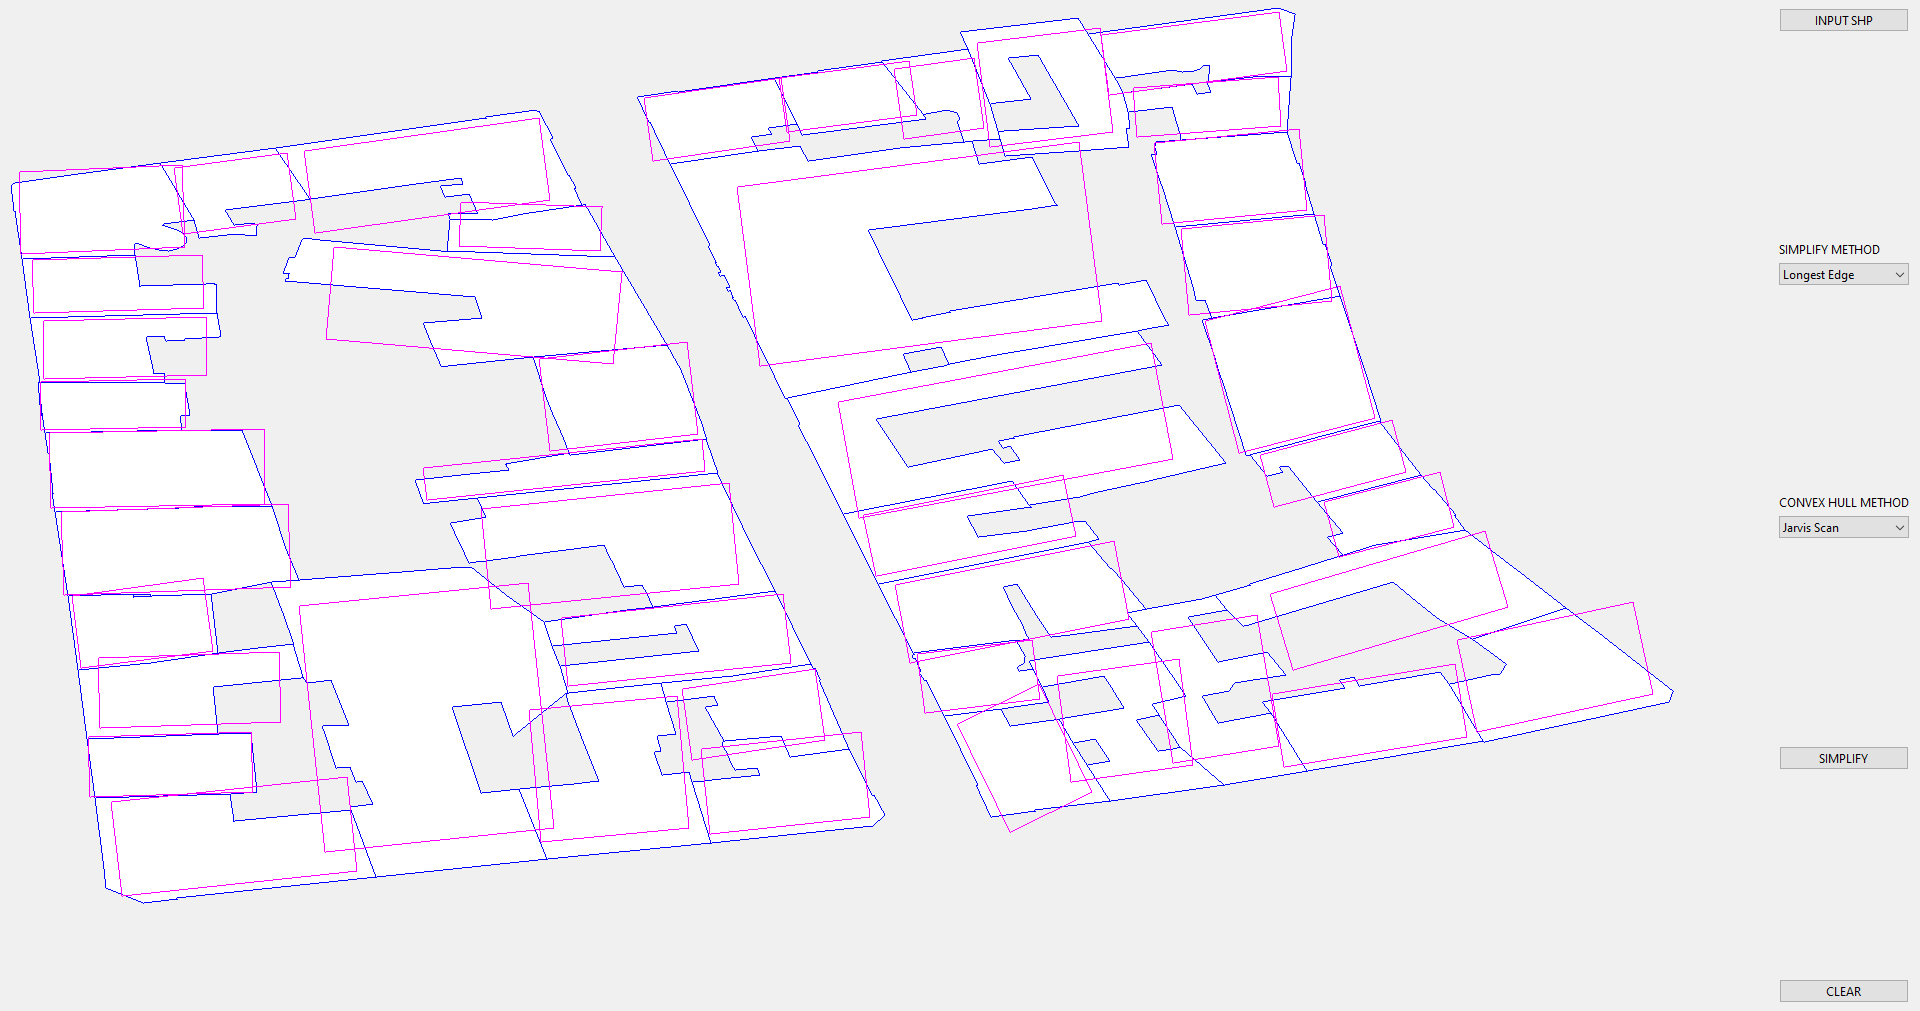
\includegraphics[width=15.65cm, height=8.2cm]{images/aplikacia2.png}
\caption{Výsledná generalizácia.}
\label{fig:obr5}
\end{figure}

%\begin{figure}[h]
    %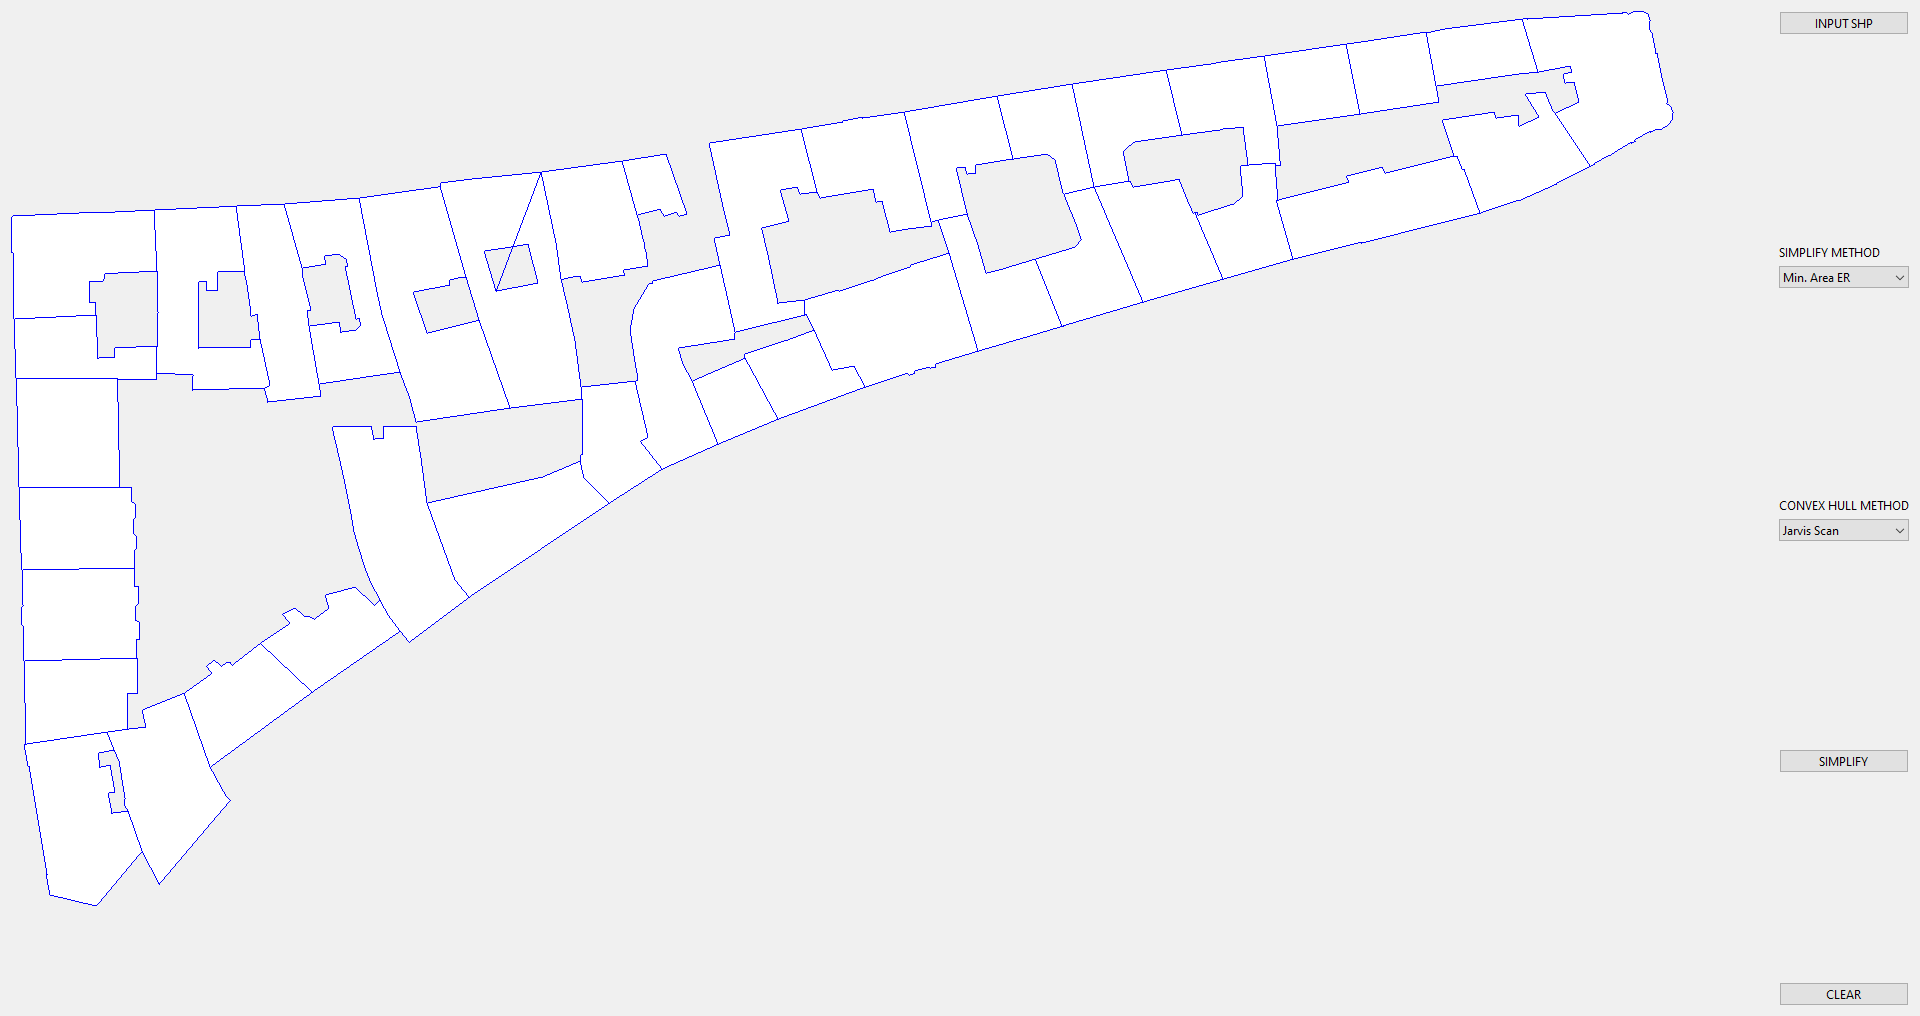
\includegraphics[width=15.65cm, height=8.2cm]{aplikacia1.png}
    %\centering
    %\caption{Užívateľské rozhranie po načítaní dát, zdroj: autor.}
    %\label{fig:obr4}
%\end{figure}

\noindent Po nahratí dát si užívateľ môže z combo-boxu vybrať, ktorý algoritmus chce použiť a ktorú metódu konštrukcie konvexnej obálky chce v rámci algoritmu \textit{Minumum Area Enclosing Rectangle} využiť.

\noindent Samotná generalizácia sa vykoná po kliknutí na tlačidlo \textit{SIMPLIFY} a výsledok sa zobrazí na zobrazovacej ploche (pozri Obr. \ref{fig:obr5}).

\noindent Posledné tlačidlo \textit{CLEAR} resetuje zobrazovaciu plochu.

\newpage


\section{Zhodnotenie}
V prvom rade boli všetky spomenuté algoritmy vyskúšané na objemnejších dátach, konkrétne na 505 polygónoch reprezentujúcich budovy v pražských Vinohradoch, tj. typické (pravidelné) bloky budov.  
Výsledky generalizácie tohto datasetu sú na Obr. \ref{fig:obr6}, Obr. \ref{fig:obr7}, Obr. \ref{fig:obr8}, Obr. \ref{fig:obr9}.
\begin{figure}[h]
\captionsetup{justification=centering}
\centering
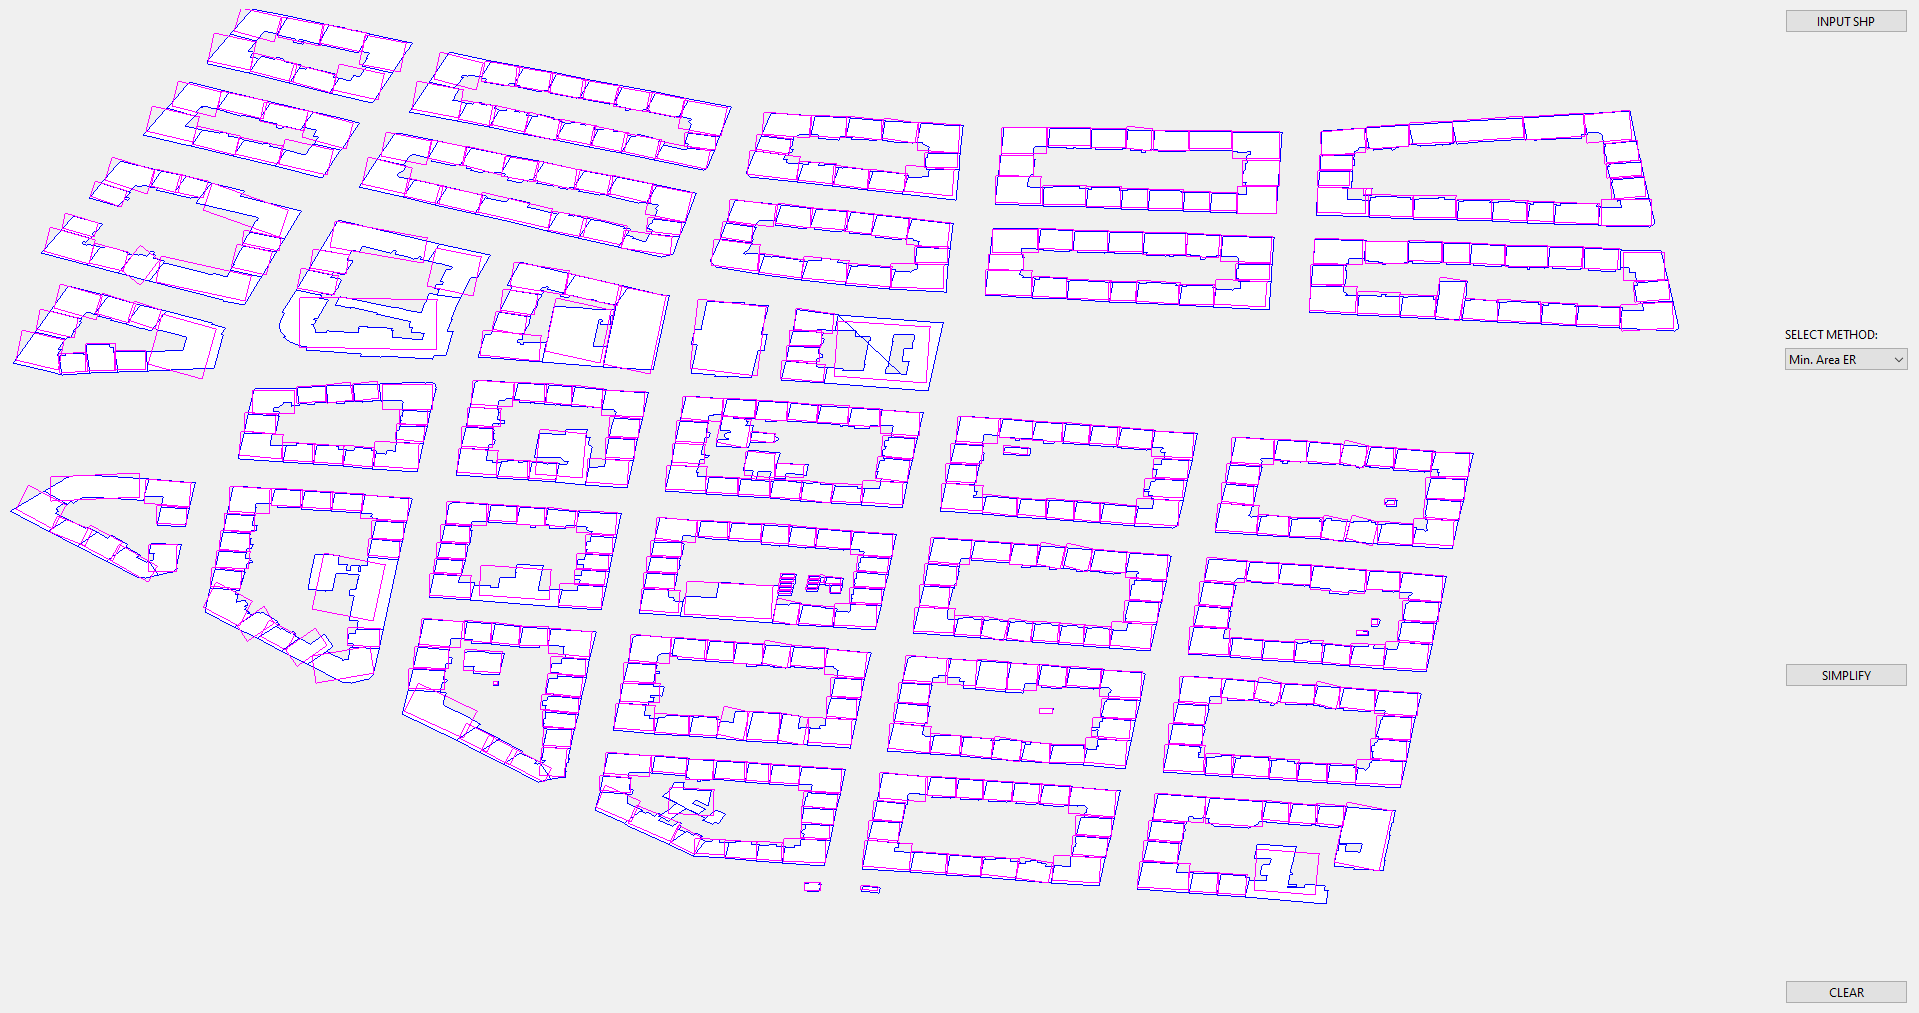
\includegraphics[width=14.65cm, height=7.2cm]{images/vinohrady_maer.png}
\caption{Generalizácia datasetu Vinohrady algoritmom \textit{Minimum Area Enclosing Rectangle}.}
\label{fig:obr6}
\end{figure}

\begin{figure}[h]
\captionsetup{justification=centering}
\centering
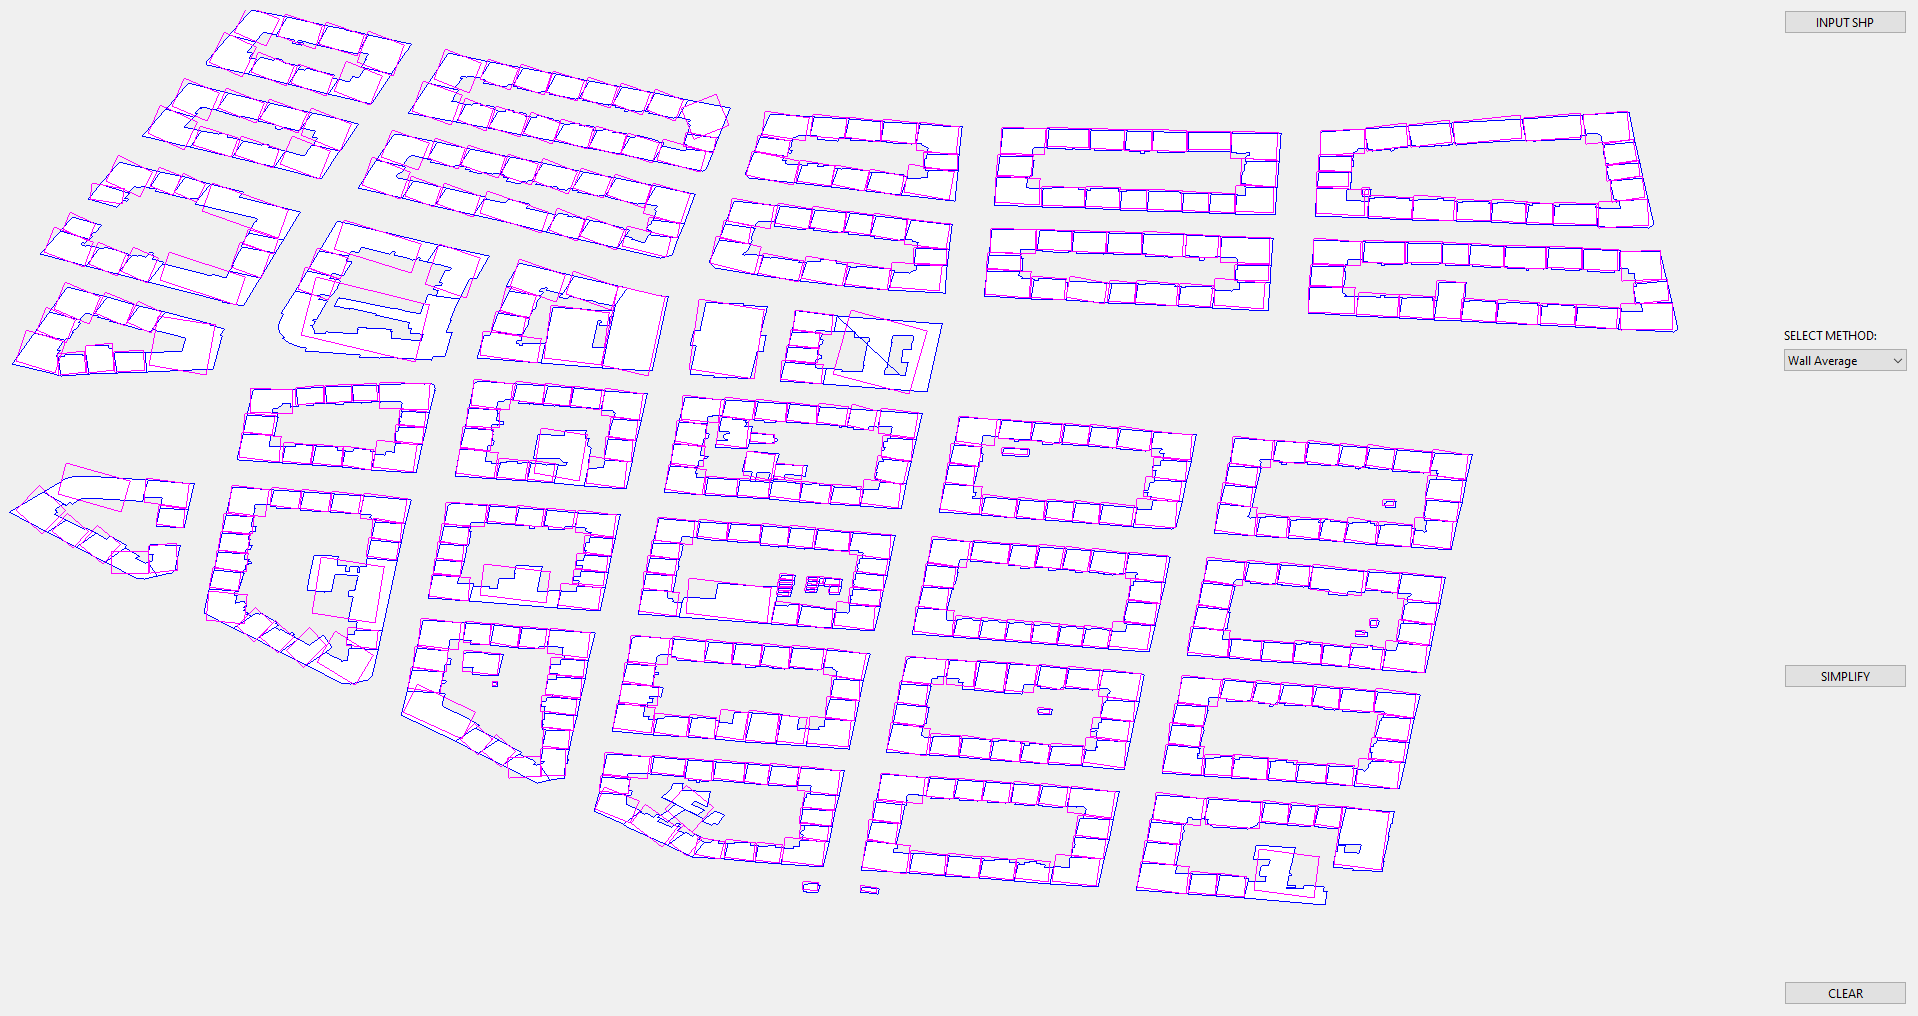
\includegraphics[width=14.65cm, height=7.2cm]{images/vinohrady_wa.png}
\caption{Generalizácia datasetu Vinohrady algoritmom \textit{Wall Average}.}
\label{fig:obr7}
\end{figure}
\newpage

\begin{figure}[h]
\captionsetup{justification=centering}
\centering
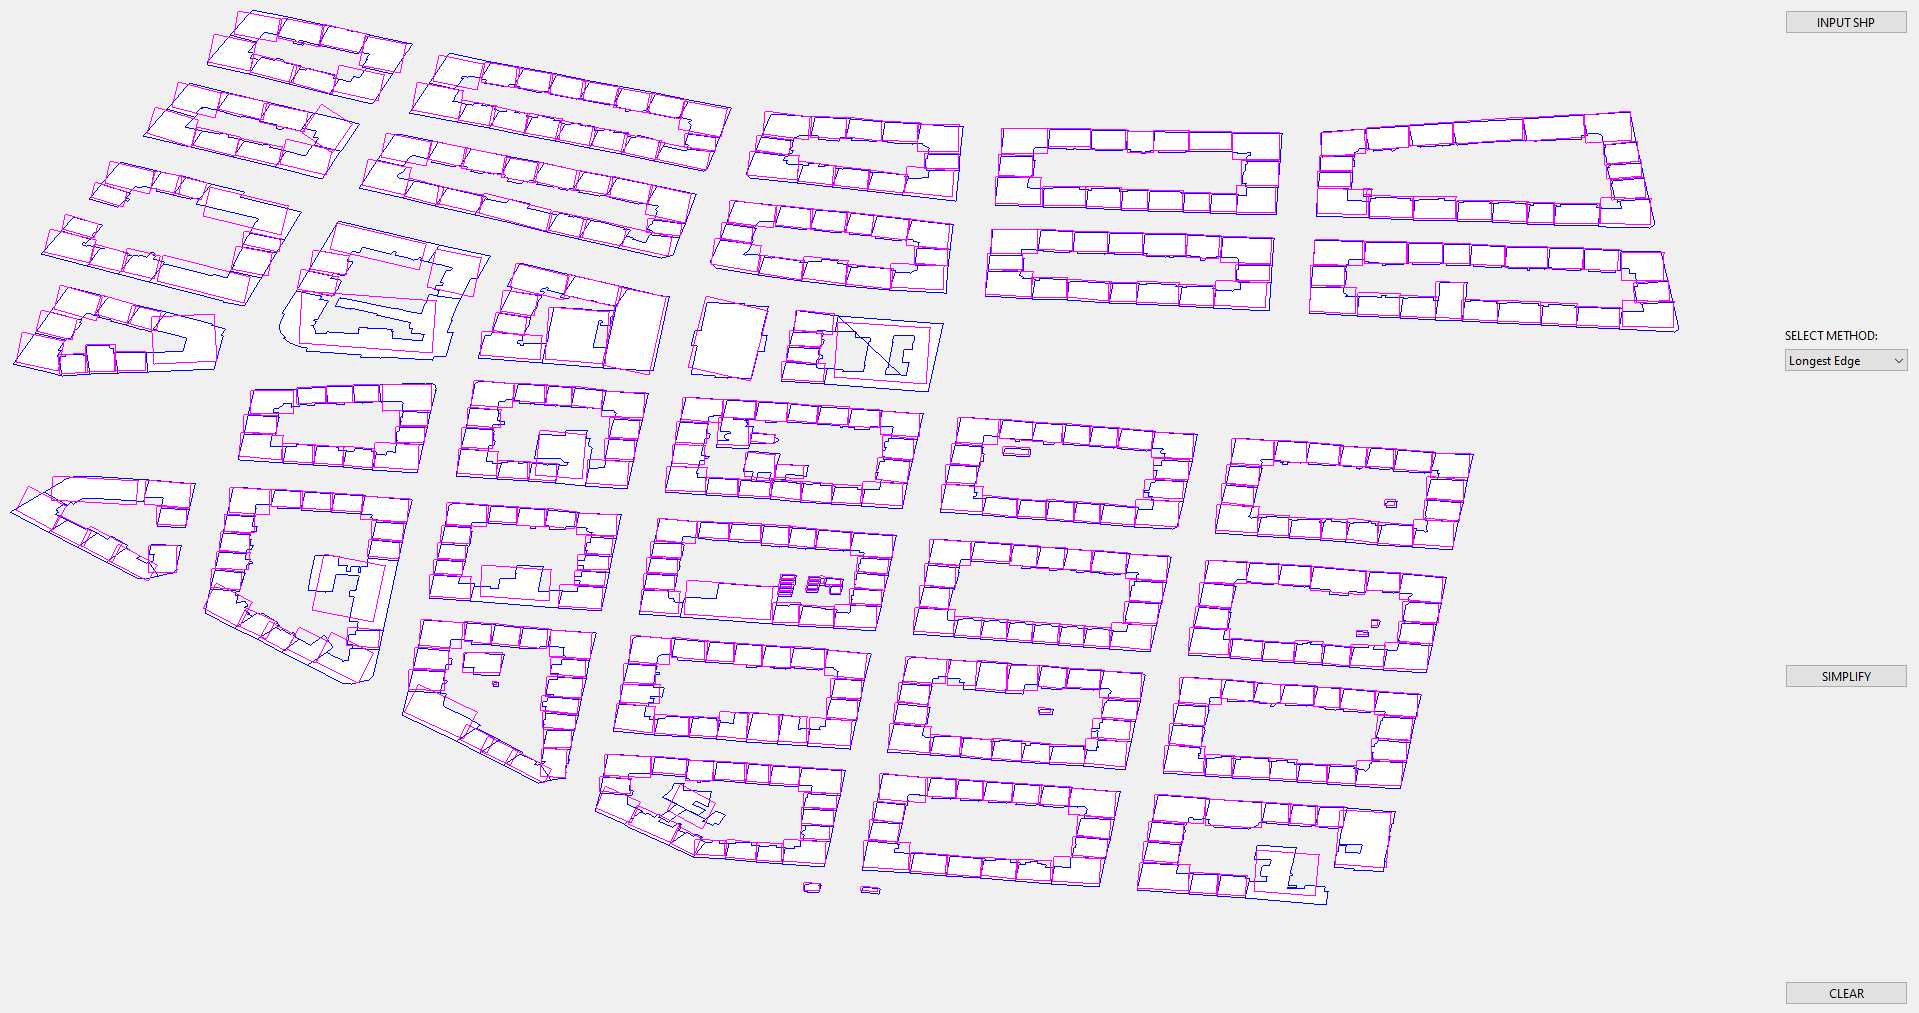
\includegraphics[width=14.65cm, height=7.2cm]{images/vinohrady_le.png}
\caption{Generalizácia datasetu Vinohrady algoritmom \textit{Longest Edge}.}
\label{fig:obr8}
\end{figure}

\begin{figure}[h]
\captionsetup{justification=centering}
\centering
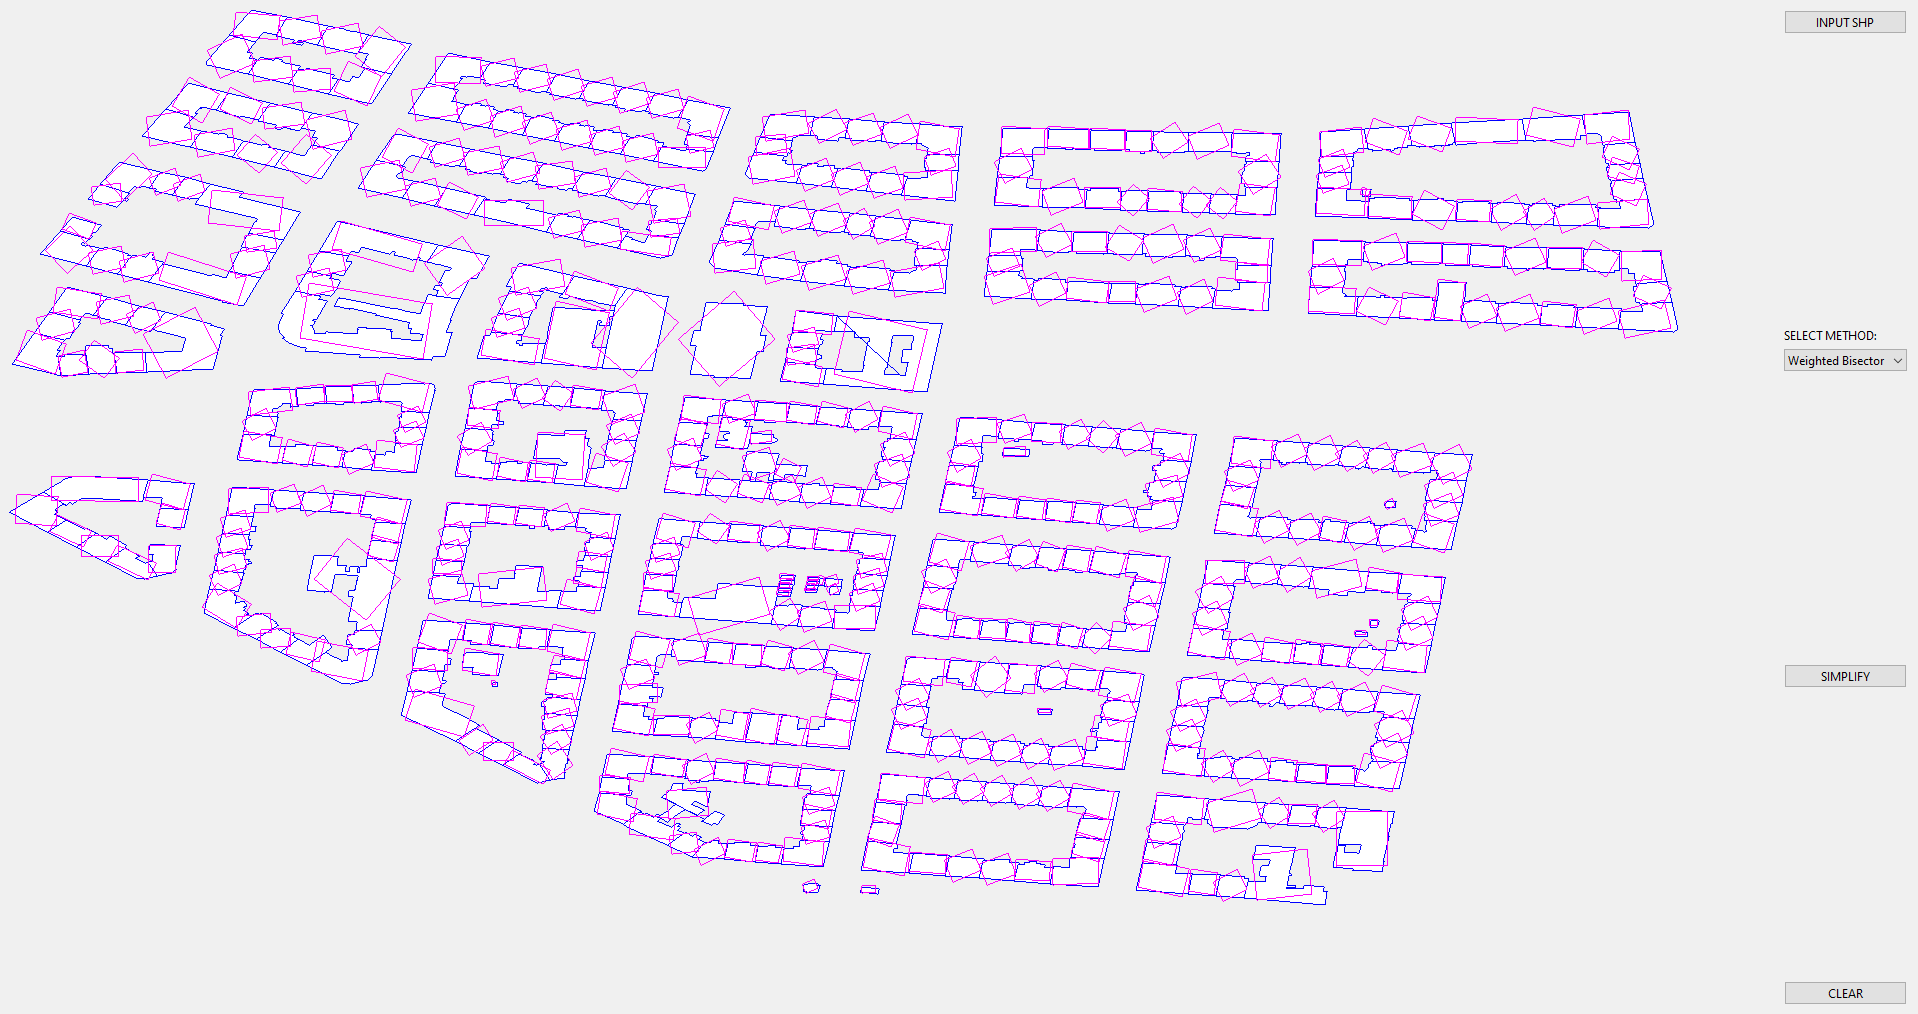
\includegraphics[width=14.65cm, height=7.2cm]{images/vinohrady_bi.png}
\caption{Generalizácia datasetu Vinohrady algoritmom \textit{Weighted Bisector}.}
\label{fig:obr9}
\end{figure}

\noindent Algoritmy \textit{Minimum Area Enclosing Rectangle}, \textit{Wall Average} a \textit{Longest Edge} tento dataset vyhodnotili veľmi podobne, rozdiely v orientácií generalizovaných budov sú viacmenej minimálne, a zároveň boli dosiahnuté uspokojivé výsledky. Algoritmus \textit{Weighted Bisector} určil orientáciu pri väčšine budov nesprávne a výsledky sú neuspokojivé. Môžeme pozorovať, že častokrát budovy obdĺžnikového alebo štvorcového tvaru sú nesprávne natočené o cca 45°. Možnou príčinou chybných výsledkov tohto algoritmu je jeho nesprávna implementácia.

\newpage
Druhým testovacím datasetom bol dataset obsahujúci množstvo zaujímavých tvarov budov. Výsledky jeho generalizácie sú na Obr. \ref{fig:obr10}, Obr. \ref{fig:obr11}, Obr. \ref{fig:obr12}, Obr. \ref{fig:obr13}.

\begin{figure}[h]
\captionsetup{justification=centering}
\centering
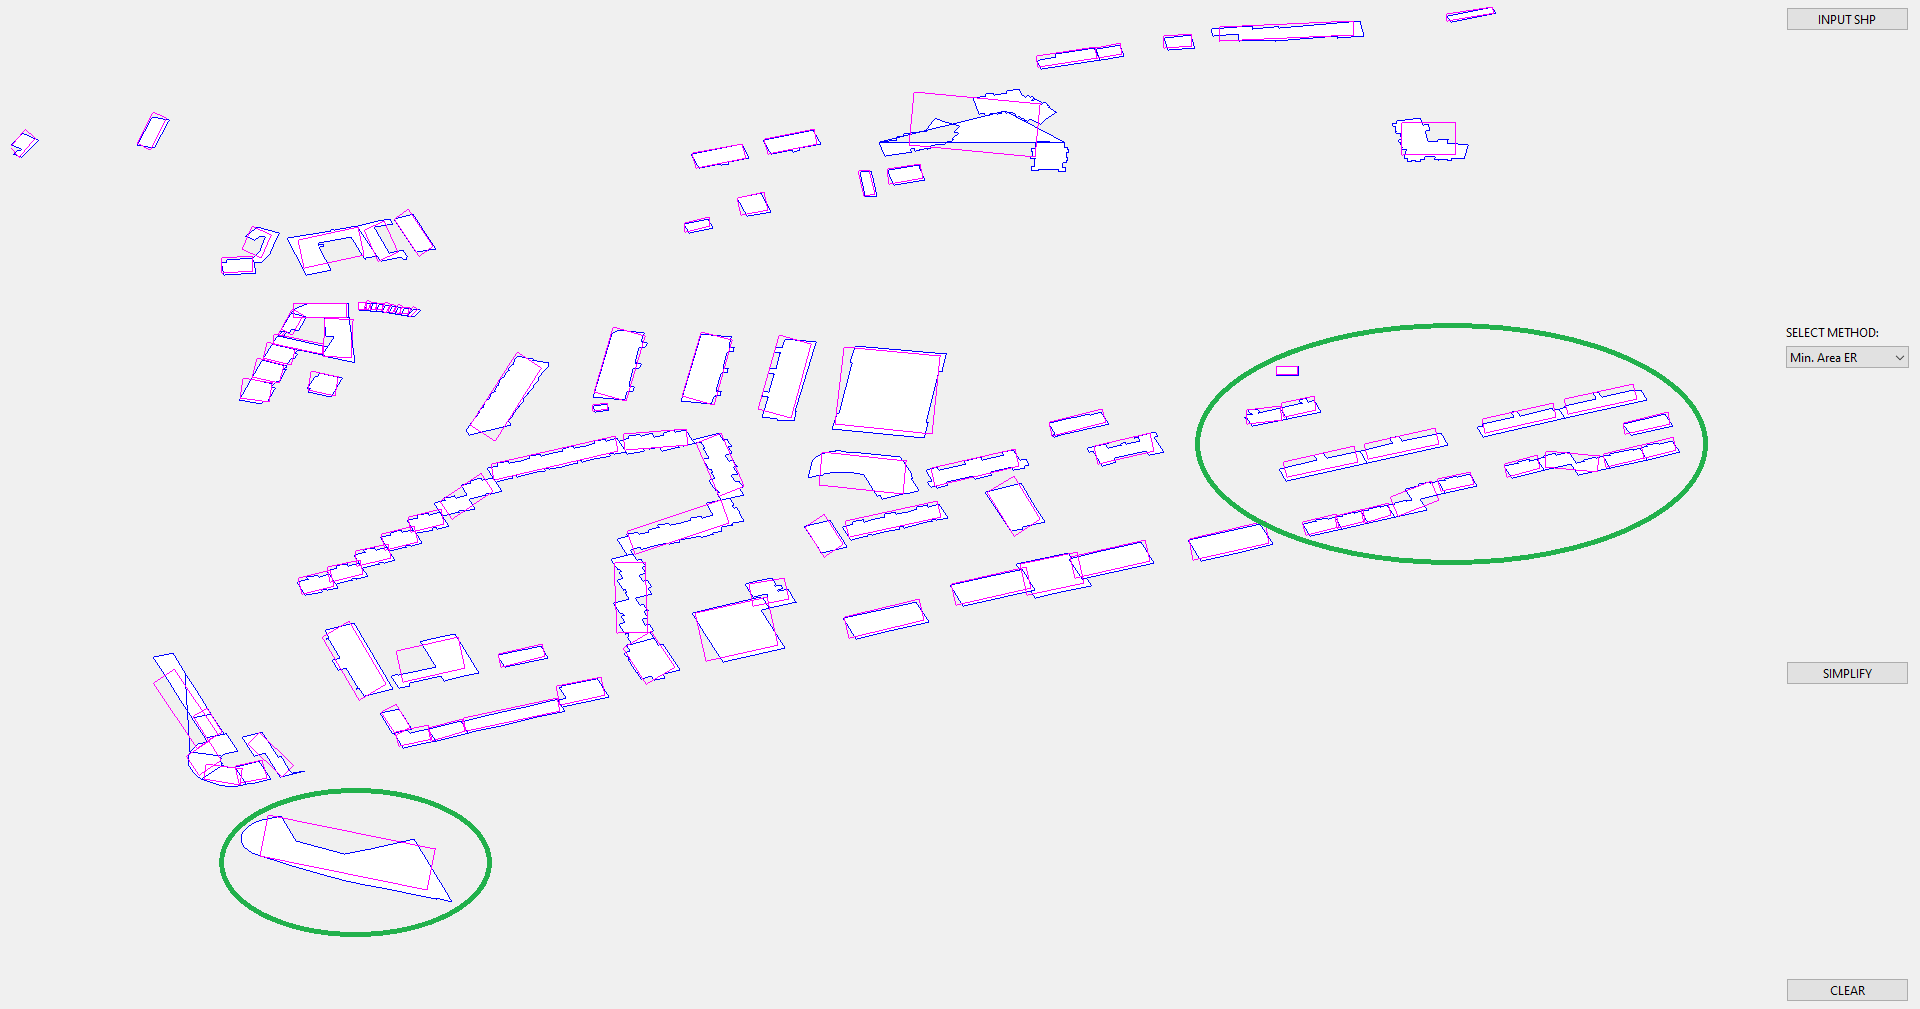
\includegraphics[width=14.65cm, height=7.2cm]{images/liben_maer.png}
\caption{Generalizácia datasetu Libeň algoritmom \textit{Minimum Area Enclosing Rectangle}.}
\label{fig:obr10}
\end{figure}

\begin{figure}[h]
\captionsetup{justification=centering}
\centering
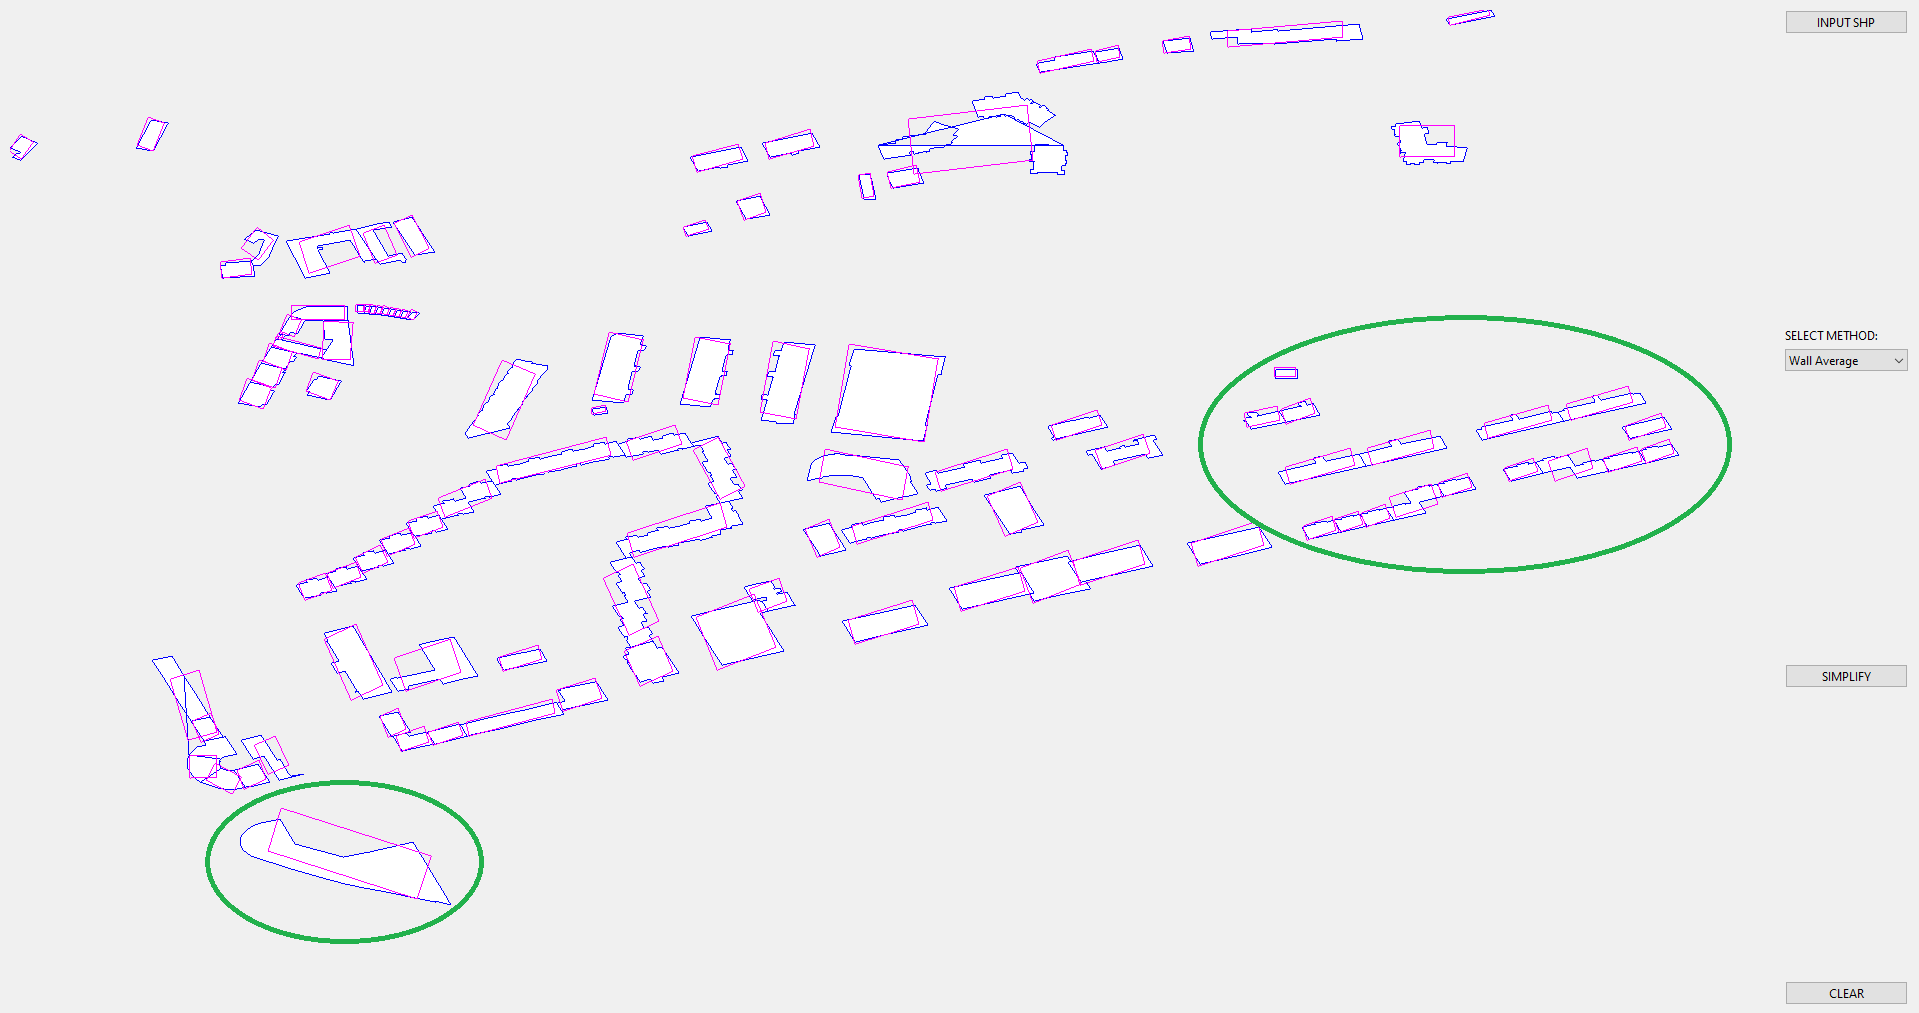
\includegraphics[width=14.65cm, height=7.2cm]{images/liben_wa.png}
\caption{Generalizácia datasetu Libeň algoritmom \textit{Wall Average}.}
\label{fig:obr11}
\end{figure}
\newpage

\begin{figure}[h]
\captionsetup{justification=centering}
\centering
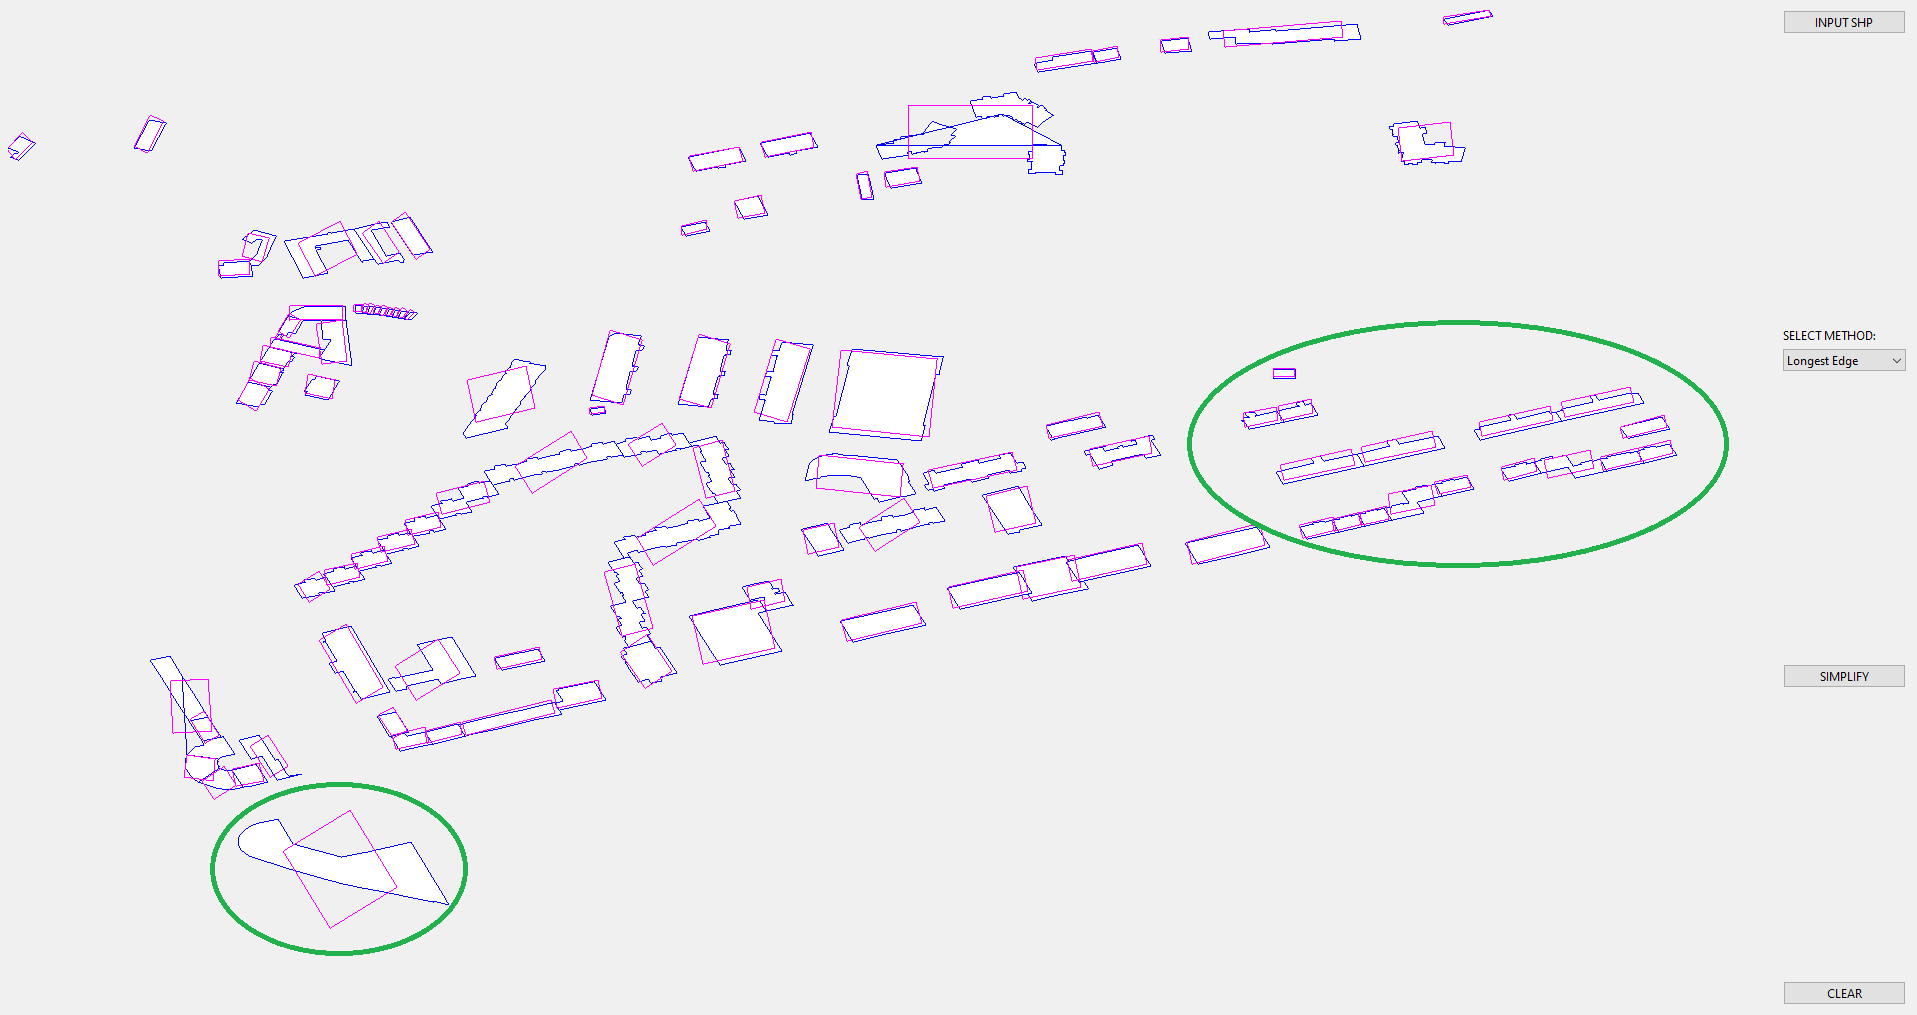
\includegraphics[width=14.65cm, height=7.2cm]{images/liben_le.png}
\caption{Generalizácia datasetu Libeň algoritmom \textit{Longest Edge}.}
\label{fig:obr12}
\end{figure}

\begin{figure}[h]
\captionsetup{justification=centering}
\centering
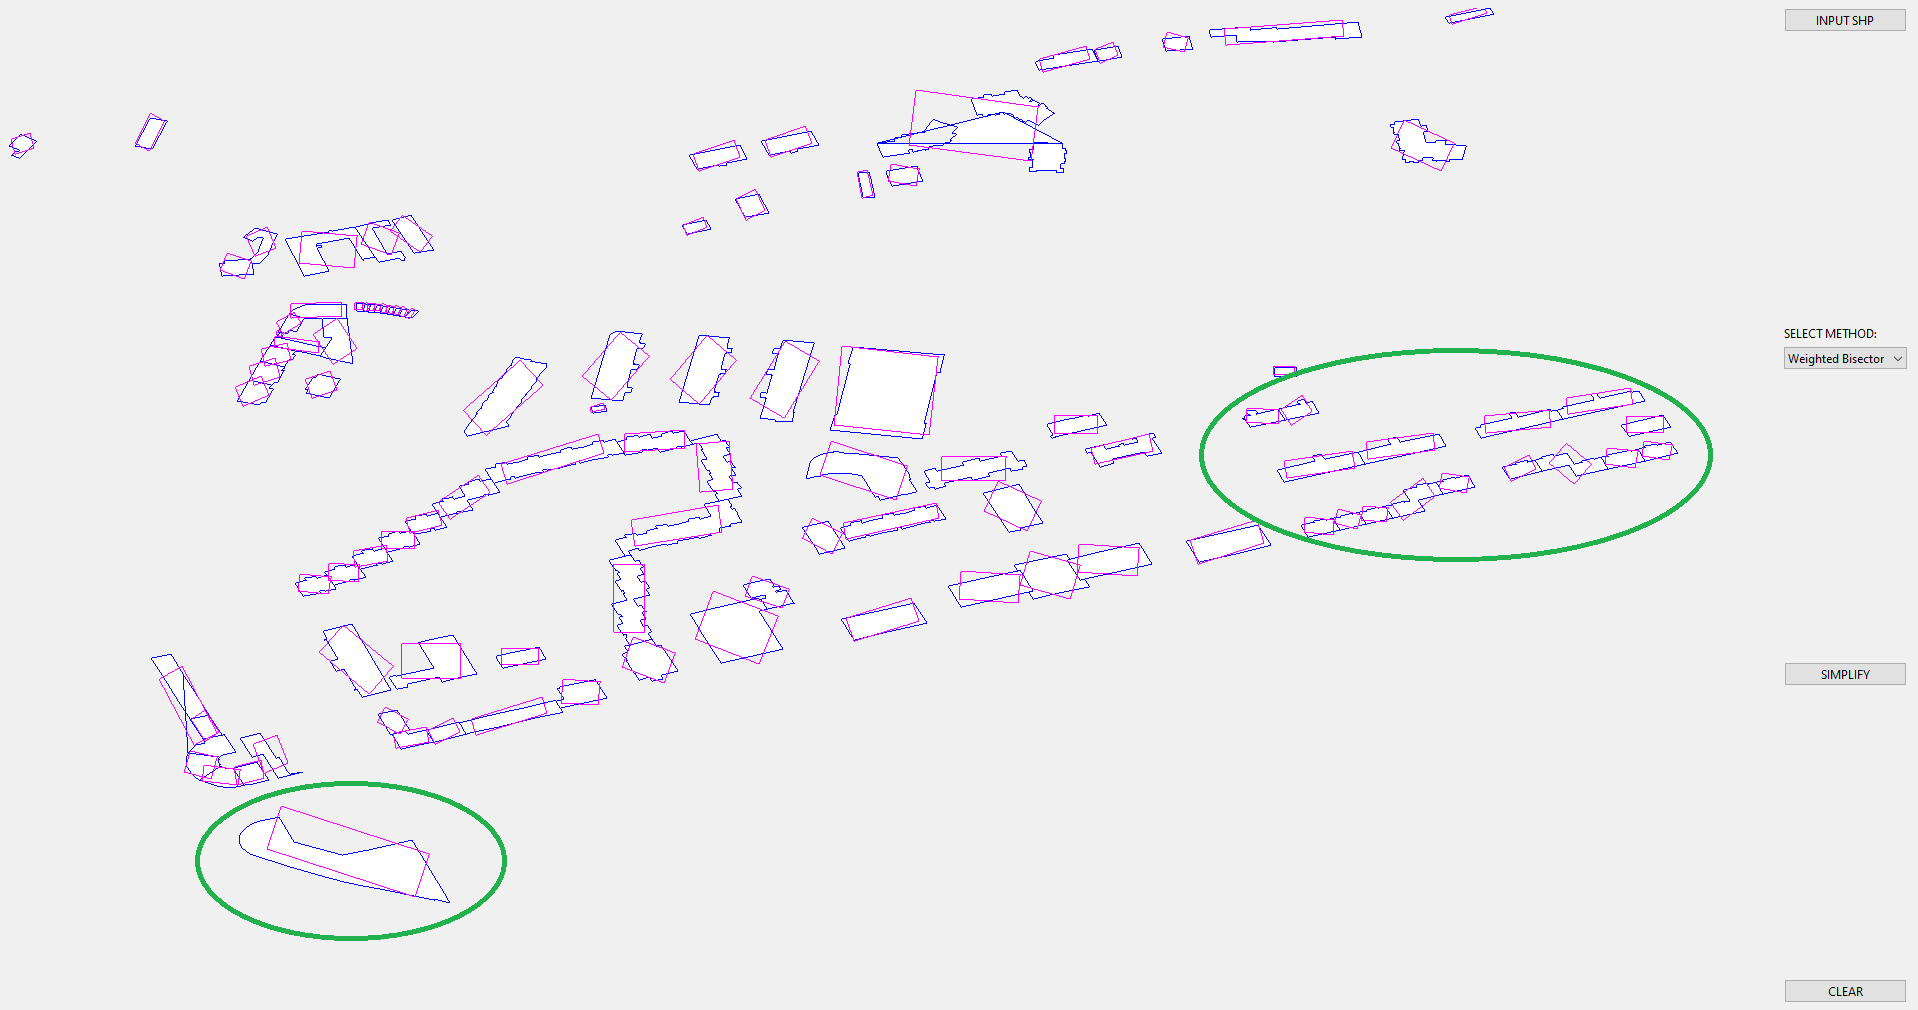
\includegraphics[width=14.65cm, height=7.2cm]{images/liben_bi.png}
\caption{Generalizácia datasetu Libeň algoritmom \textit{Weighted Bisector}.}
\label{fig:obr13}
\end{figure}

\noindent V pravej časti datasetu, kde sa nachádzajú budovy podlhovastého tvaru (zvýraznené) došlo ku najkvalitnejšej generalizácií algoritmom \textit{Longest Edge}, ktorý ale pre zvýraznenú budovu iregulárneho tvaru (budova v ľavom dolnom rohu) nedosiahol uspokojivý výsledok. S tou si najlepšie poradil prekvapujúco \textit{Weighted Bisector}, kvalitne mu sekunduje \textit{Wall Average}. Nutno dodať, že generalizácia \textit{Weighted Bisector} trvá dlhší čas v porovnaní s ostatnými algoritmami.
\newpage

Pri treťom datasete bolo cieľom demonštrovať chovanie algoritmov pri budovách zaobleného tvaru (napr. štadióny). Výsledky pre jednotlivé algoritmy sú na Obr. \ref{fig:obr14}, Obr. \ref{fig:obr15}, Obr. \ref{fig:obr16}, Obr. \ref{fig:obr17}.

\begin{figure}[h]
\captionsetup{justification=centering}
\centering
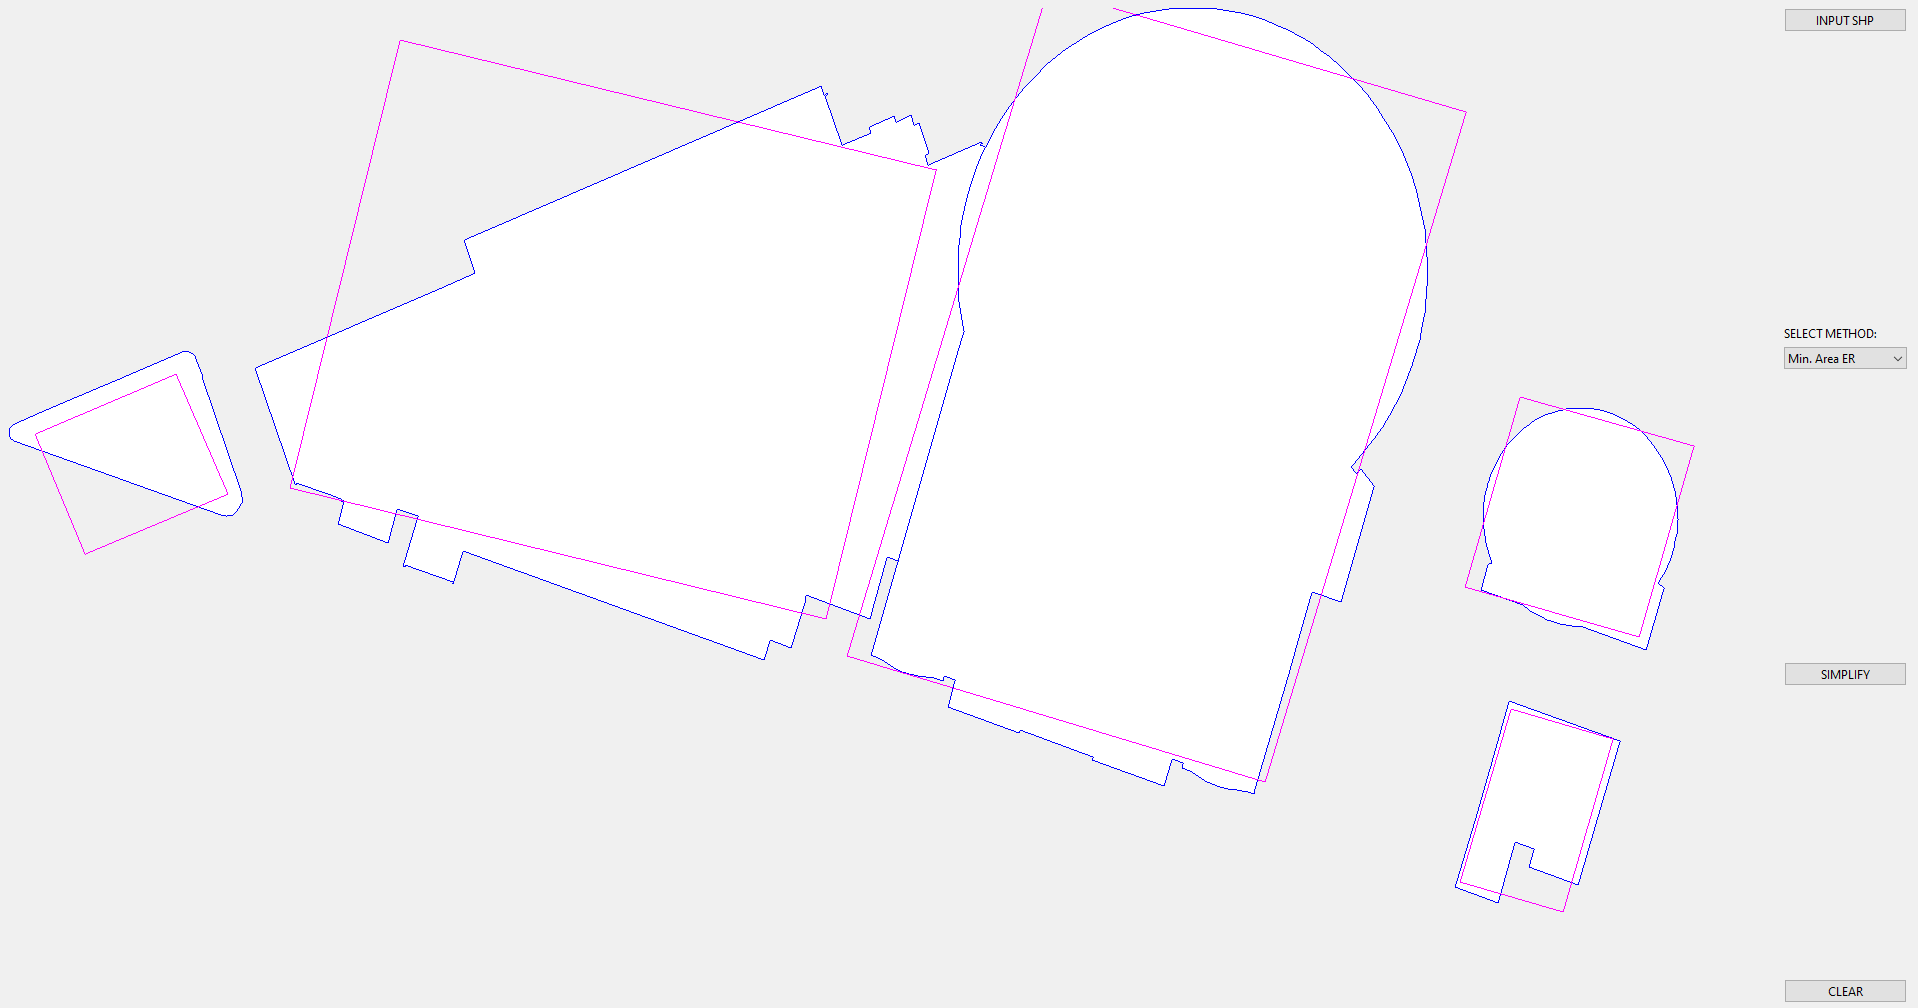
\includegraphics[width=14.65cm, height=7.2cm]{images/stadion_maer.png}
\caption{Generalizácia datasetu Štadióny algoritmom \textit{Minimum Area Enclosing Rectangle}.}
\label{fig:obr14}
\end{figure}

\begin{figure}[h]
\captionsetup{justification=centering}
\centering
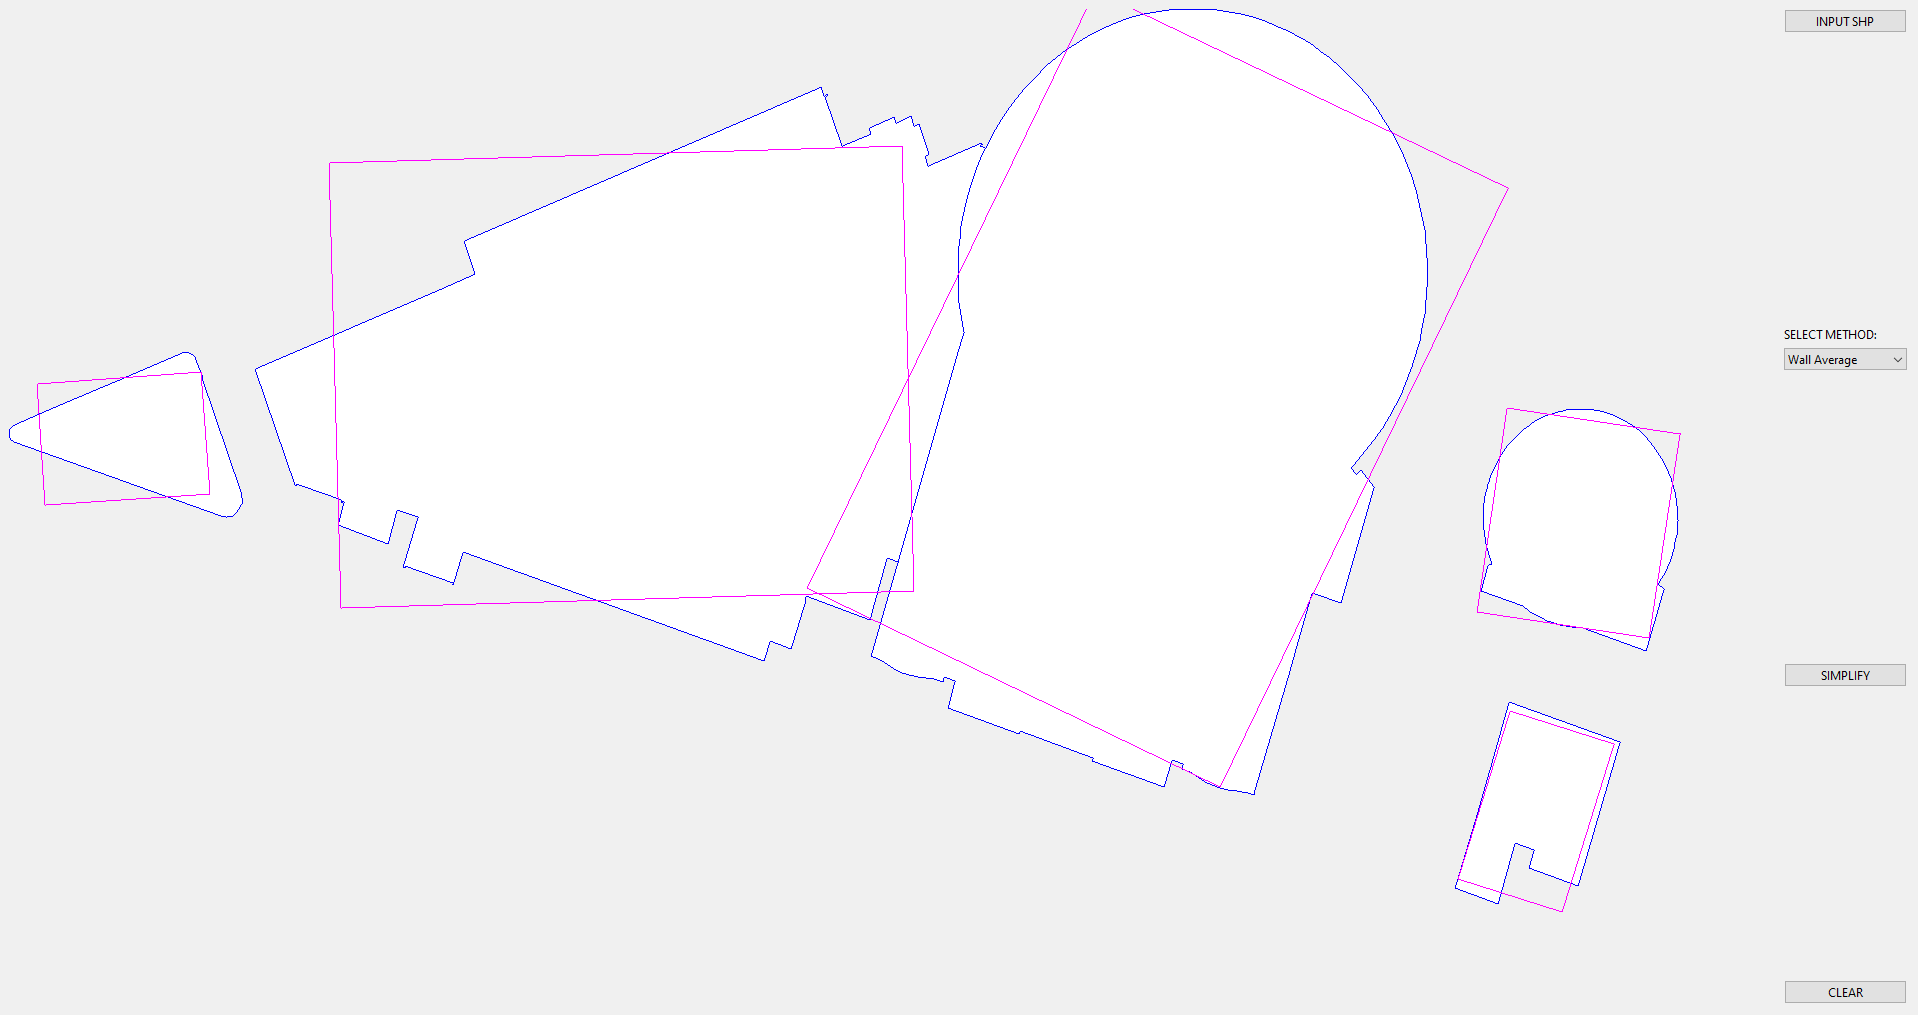
\includegraphics[width=14.65cm, height=7.2cm]{images/stadion_wa.png}
\caption{Generalizácia datasetu Štadióny algoritmom \textit{Wall Average}.}
\label{fig:obr15}
\end{figure}
\newpage

\begin{figure}[h]
\captionsetup{justification=centering}
\centering
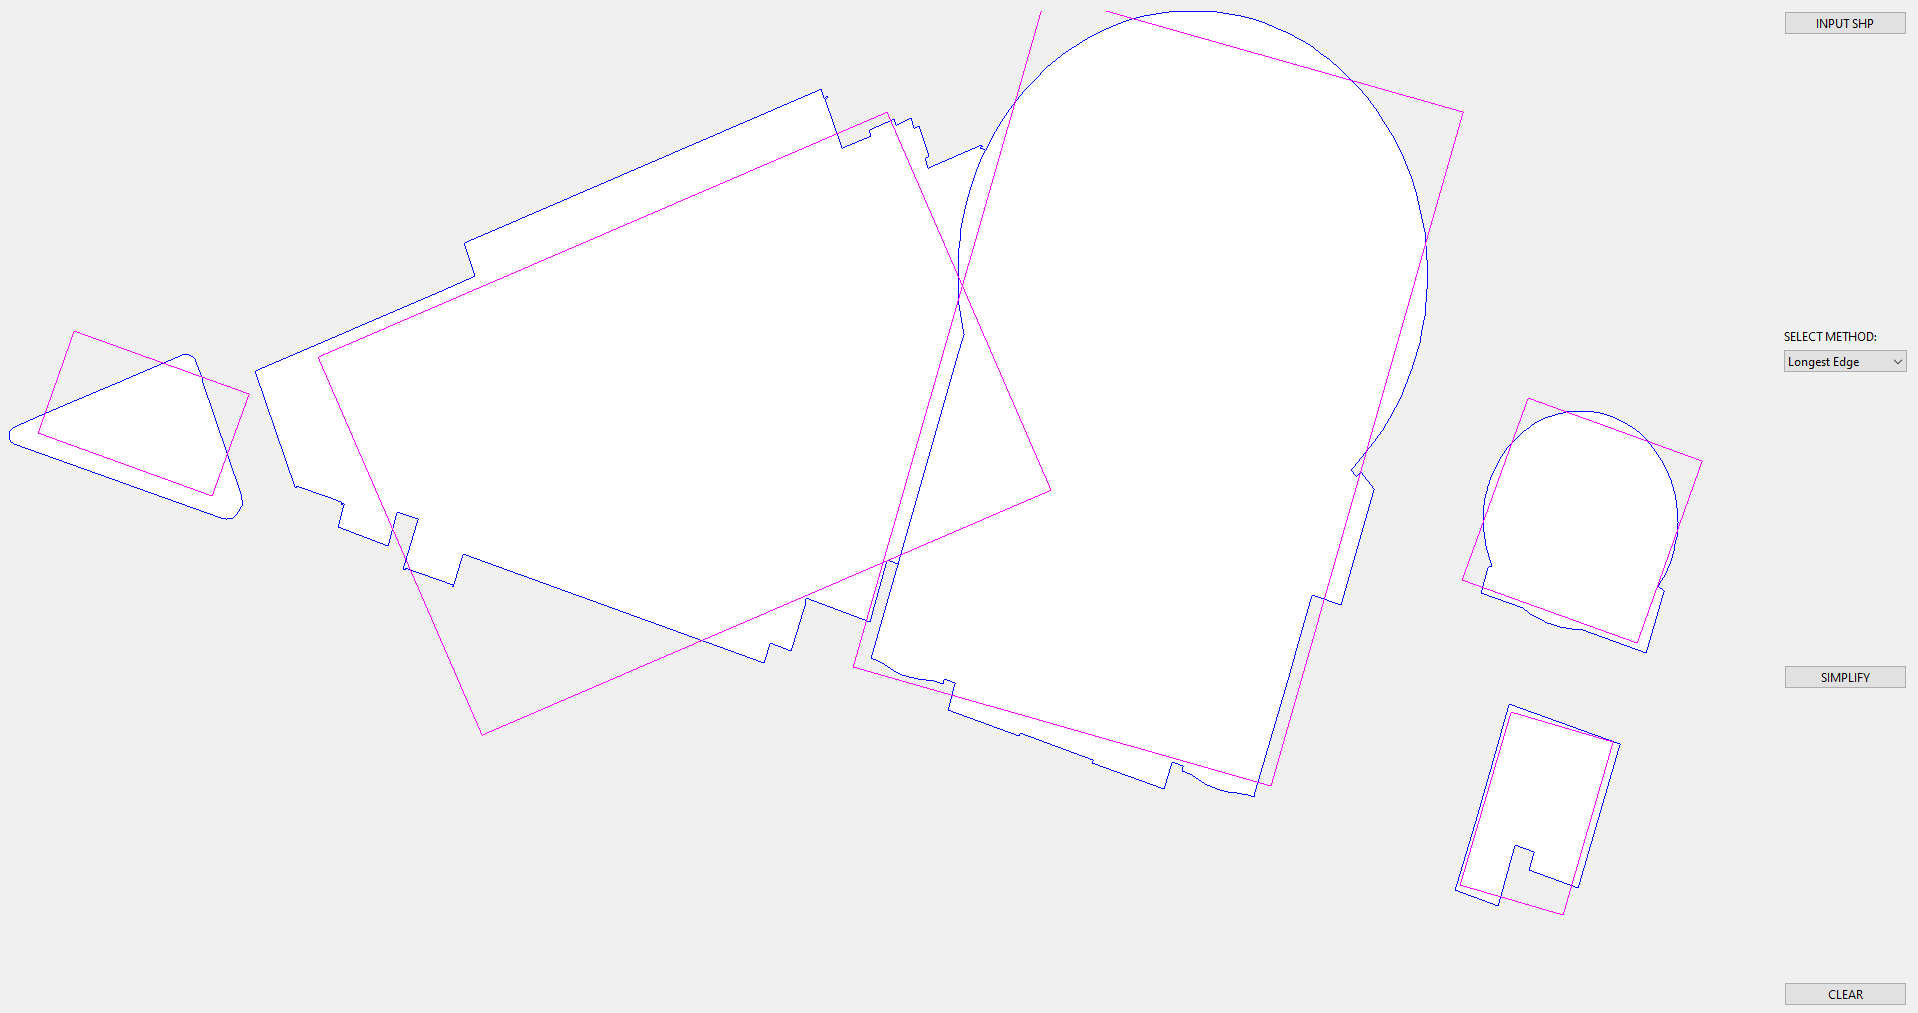
\includegraphics[width=14.65cm, height=7.2cm]{images/stadion_le.png}
\caption{Generalizácia datasetu Štadióny algoritmom \textit{Longest Edge}.}
\label{fig:obr16}
\end{figure}

\begin{figure}[h]
\captionsetup{justification=centering}
\centering
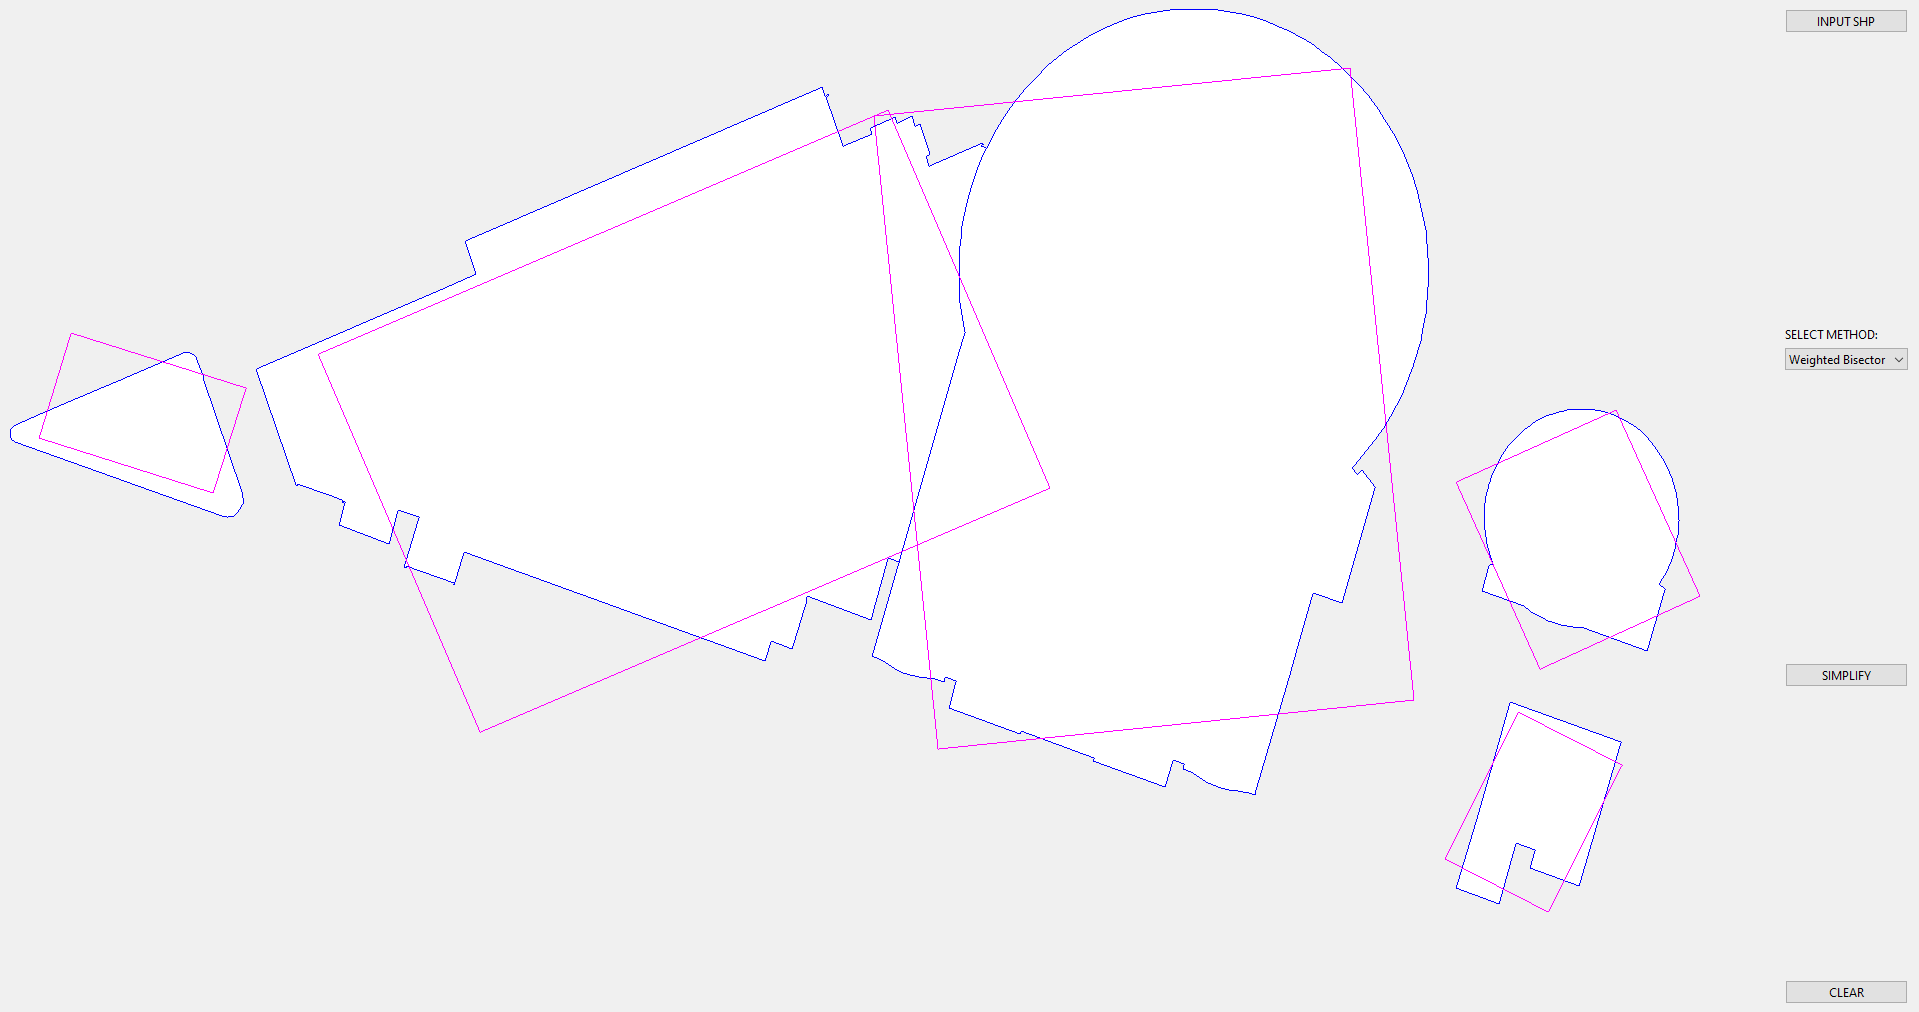
\includegraphics[width=14.65cm, height=7.2cm]{images/stadion_bi.png}
\caption{Generalizácia datasetu Štadióny algoritmom \textit{Weighted Bisector}.}
\label{fig:obr17}
\end{figure}

\noindent Najlepšie výsledky dosiahol \textit{Longest Edge}, čo sa dalo očakávať, pretože pri takýchto budovách skutočne najdlhšia hrana určuje jej orientáciu. Pre prvé dve budovy zľava (trojuholníkového tvaru) dopadli porovnateľne dobre \textit{Wall Average} a \textit{Weighted Bisector}, ktoré si ale nepodarili najlepšie so susedným štadiónom. Presne opačné závery platia pre \textit{Minimum Area Enclosing Rectangle}.

\newpage
Štvrtý dataset obsahuje budovy v tvare L a dve budovy veľmi komplexného tvaru. Výsledky sú na Obr. \ref{fig:obr18}, Obr. \ref{fig:obr19}, Obr. \ref{fig:obr20}, Obr. \ref{fig:obr21}.

\begin{figure}[h]
\captionsetup{justification=centering}
\centering
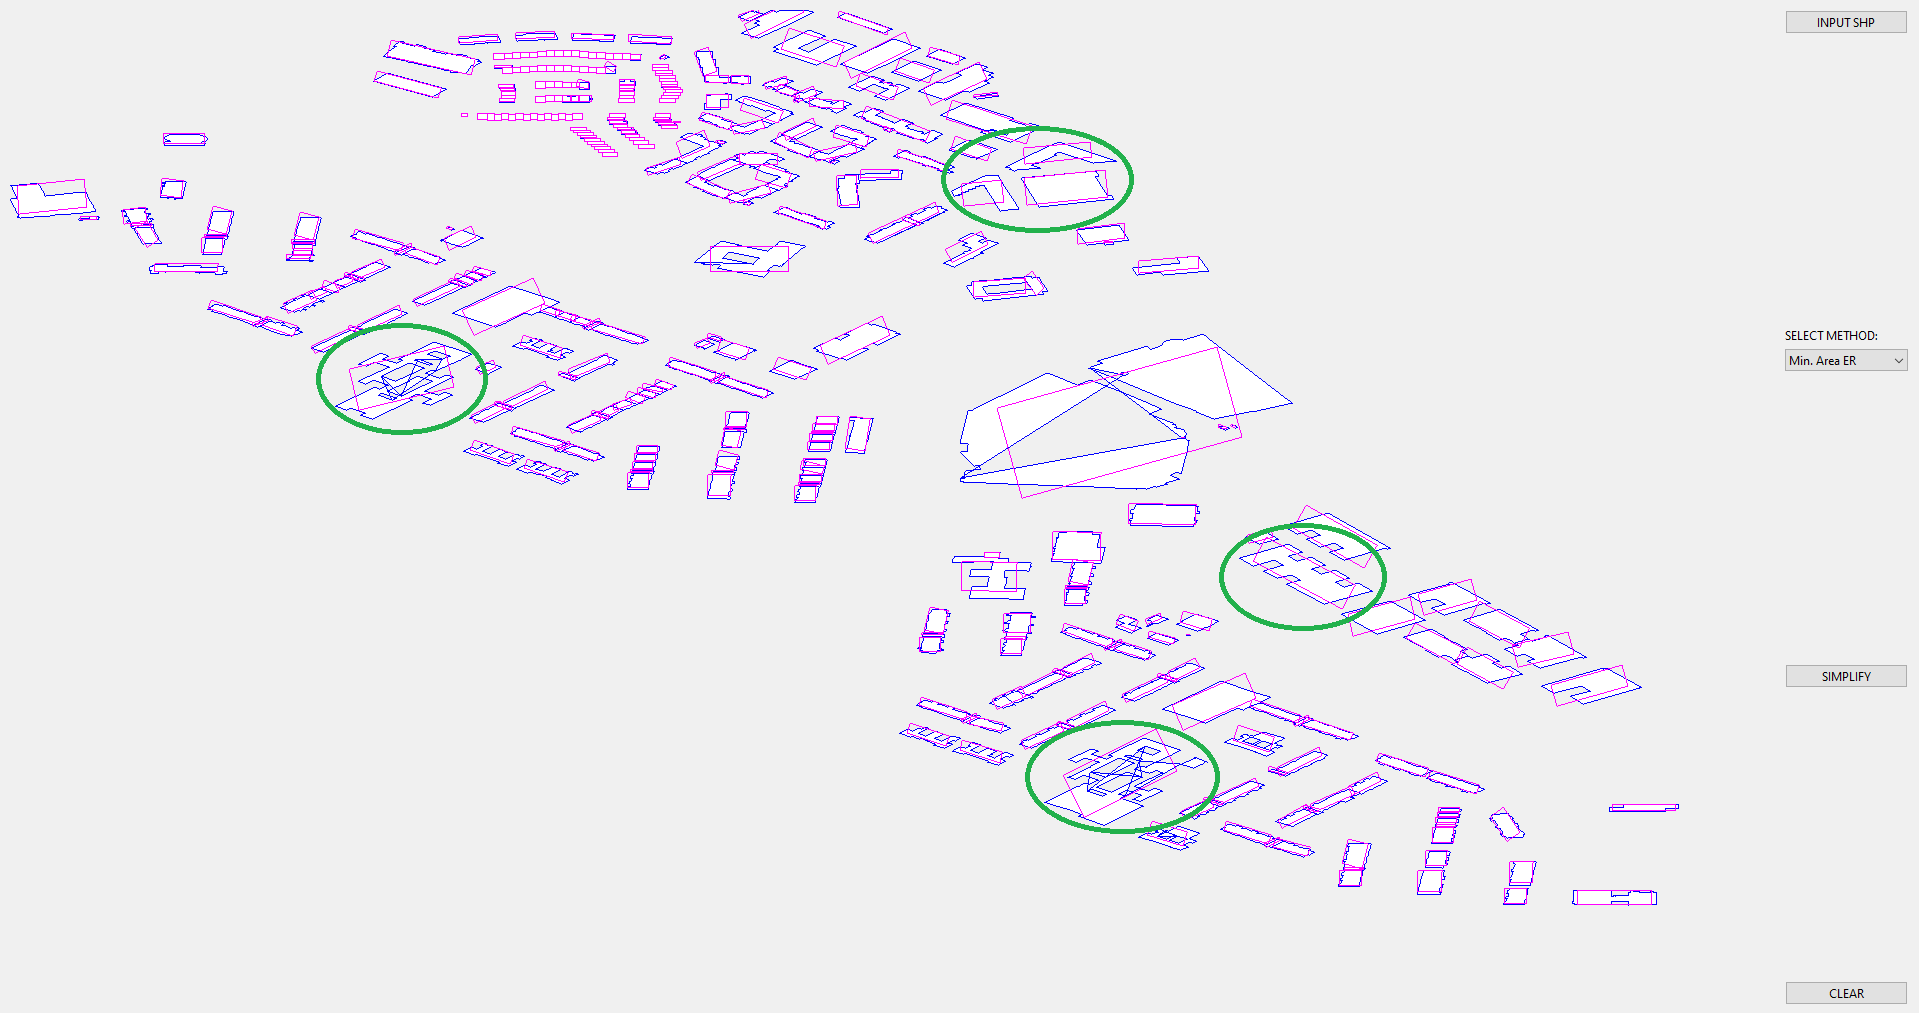
\includegraphics[width=14.65cm, height=7.5cm]{images/chodov_maer.png}
\caption{Generalizácia datasetu Chodov algoritmom \textit{Minimum Area Enclosing Rectangle}.}
\label{fig:obr18}
\end{figure}

\begin{figure}[h]
\captionsetup{justification=centering}
\centering
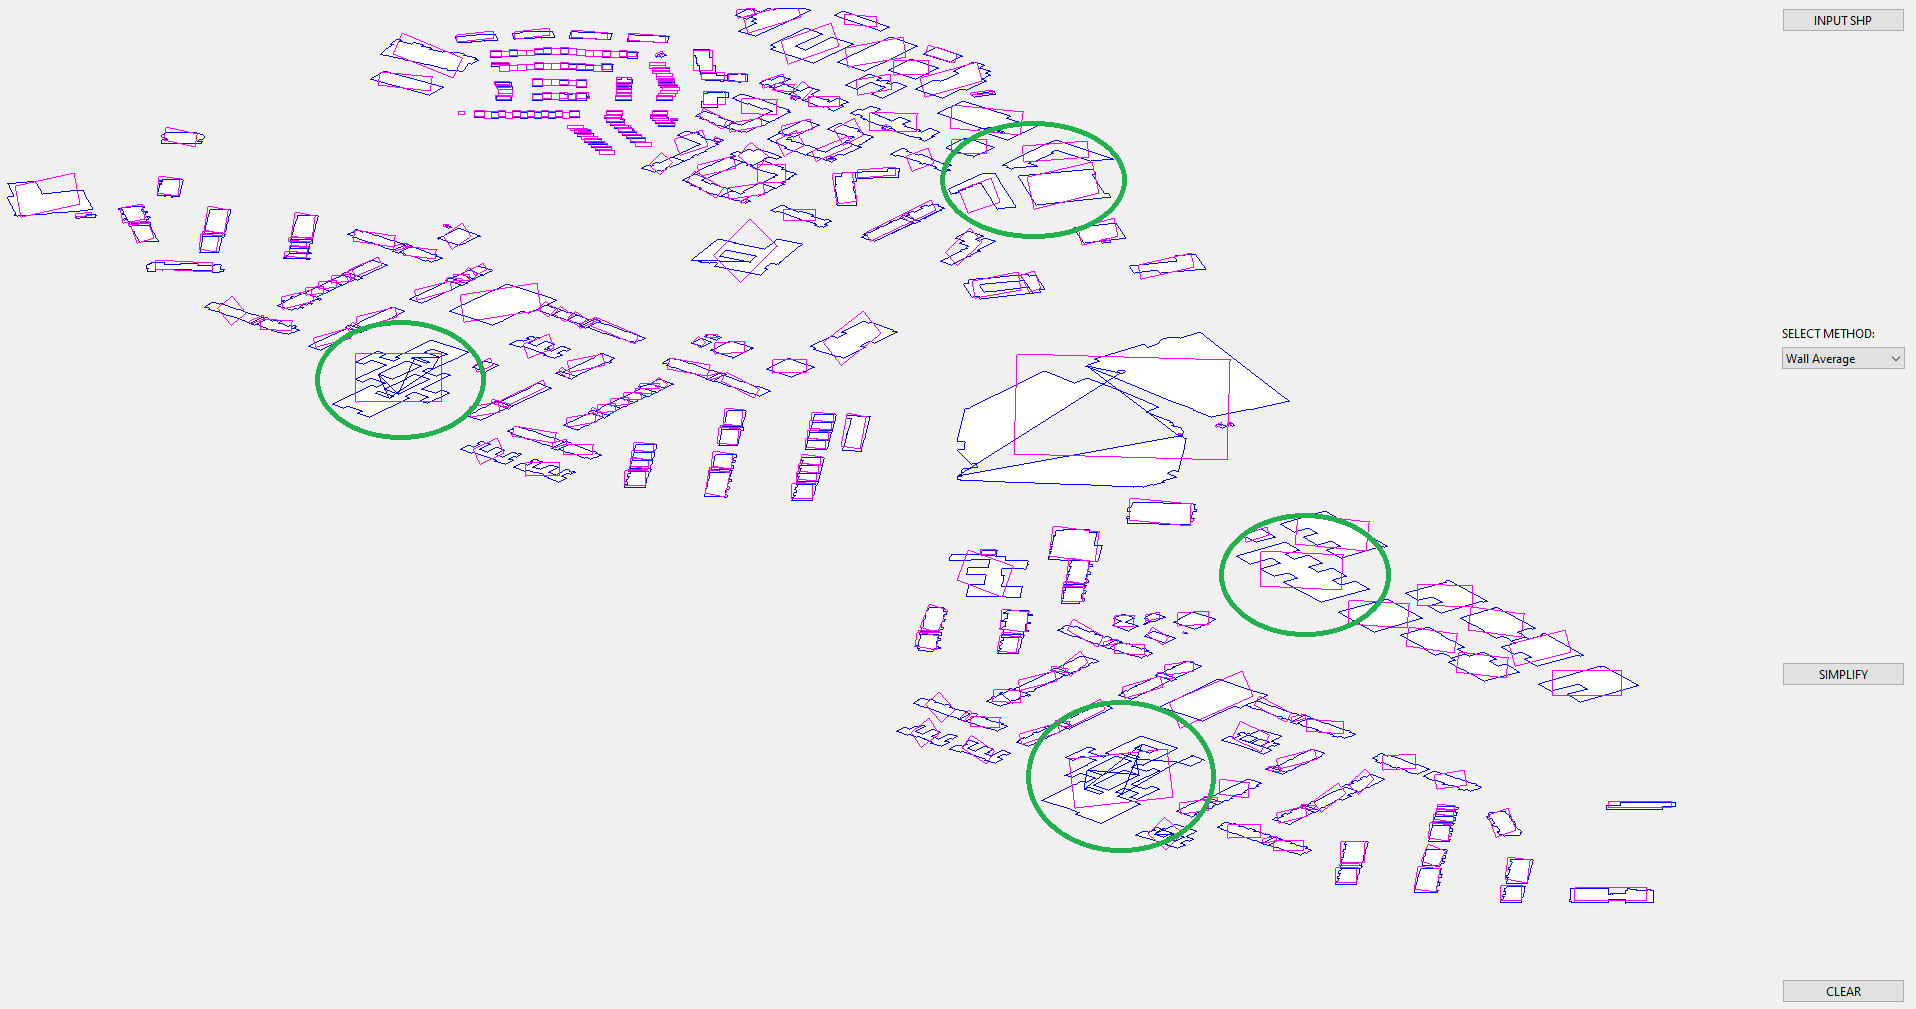
\includegraphics[width=14.65cm, height=7.5cm]{images/chodov_wa.png}
\caption{Generalizácia datasetu Chodov algoritmom \textit{Wall Average}.}
\label{fig:obr19}
\end{figure}
\newpage

\begin{figure}[h]
\captionsetup{justification=centering}
\centering
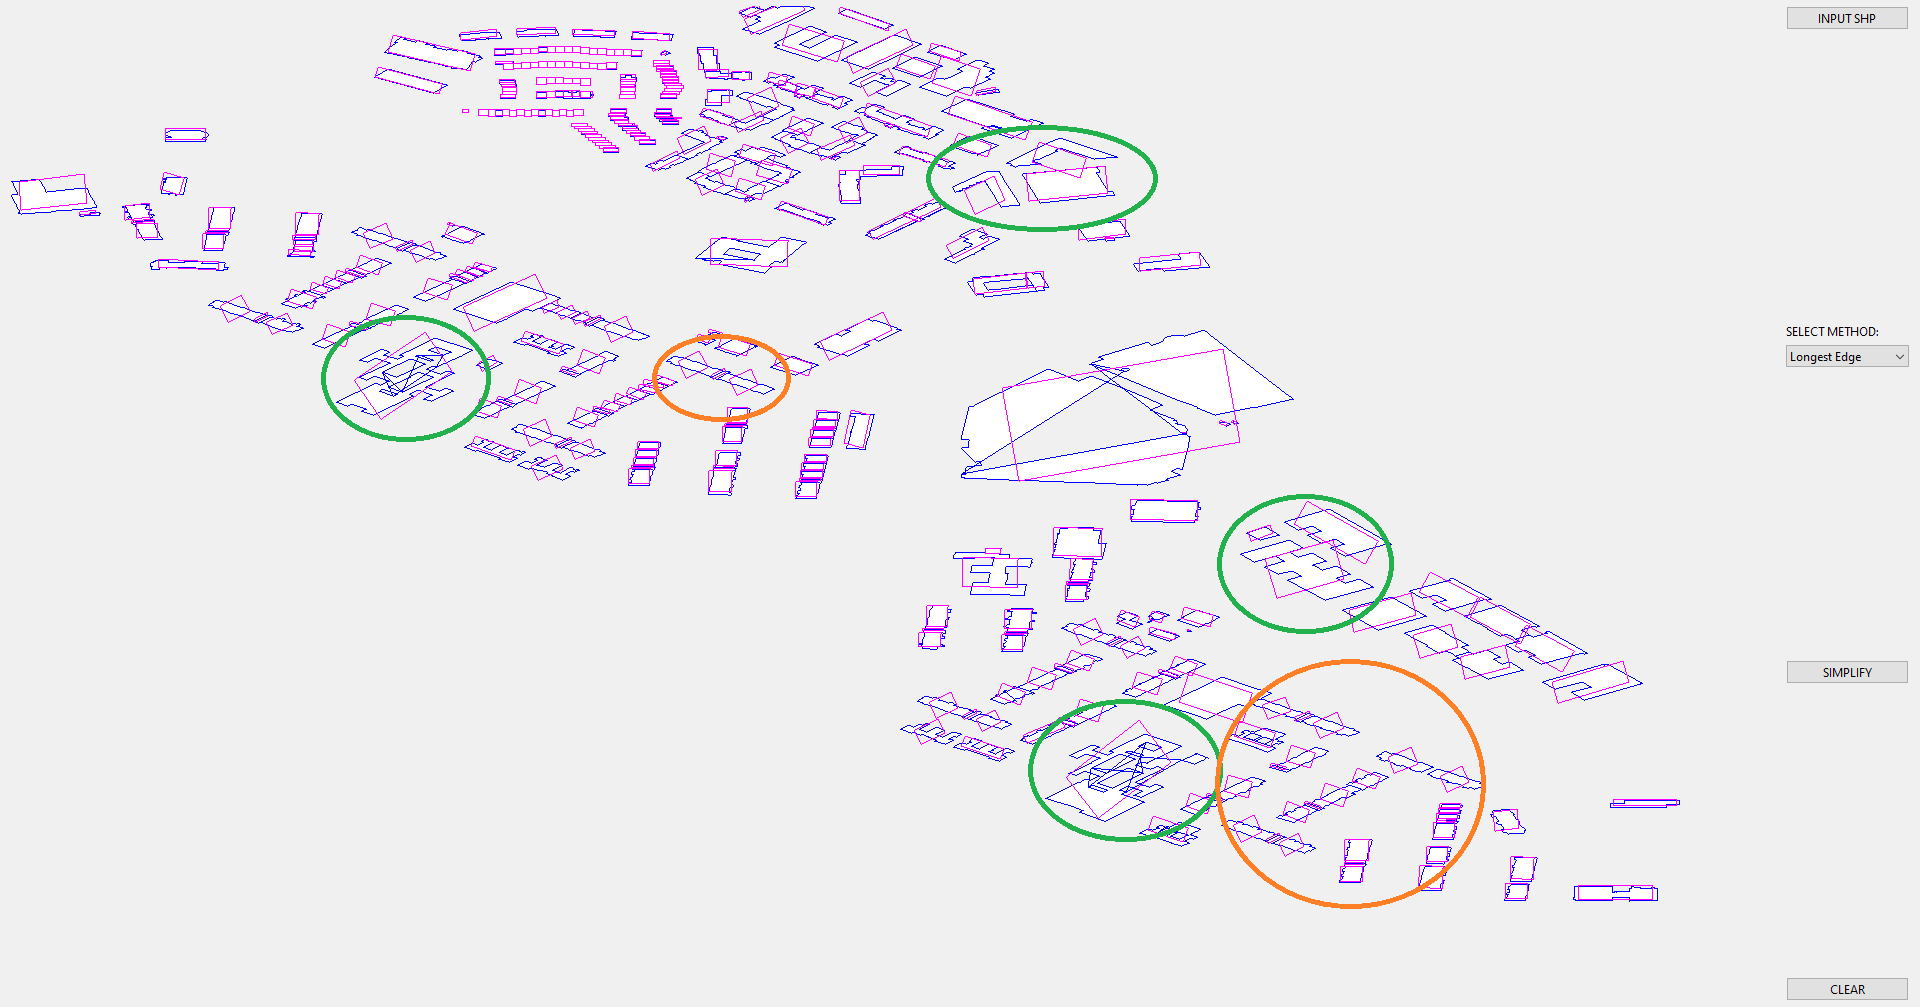
\includegraphics[width=14.65cm, height=7.5cm]{images/chodov_le.png}
\caption{Generalizácia datasetu Chodov algoritmom \textit{Longest Edge}.}
\label{fig:obr20}
\end{figure}

\begin{figure}[h]
\captionsetup{justification=centering}
\centering
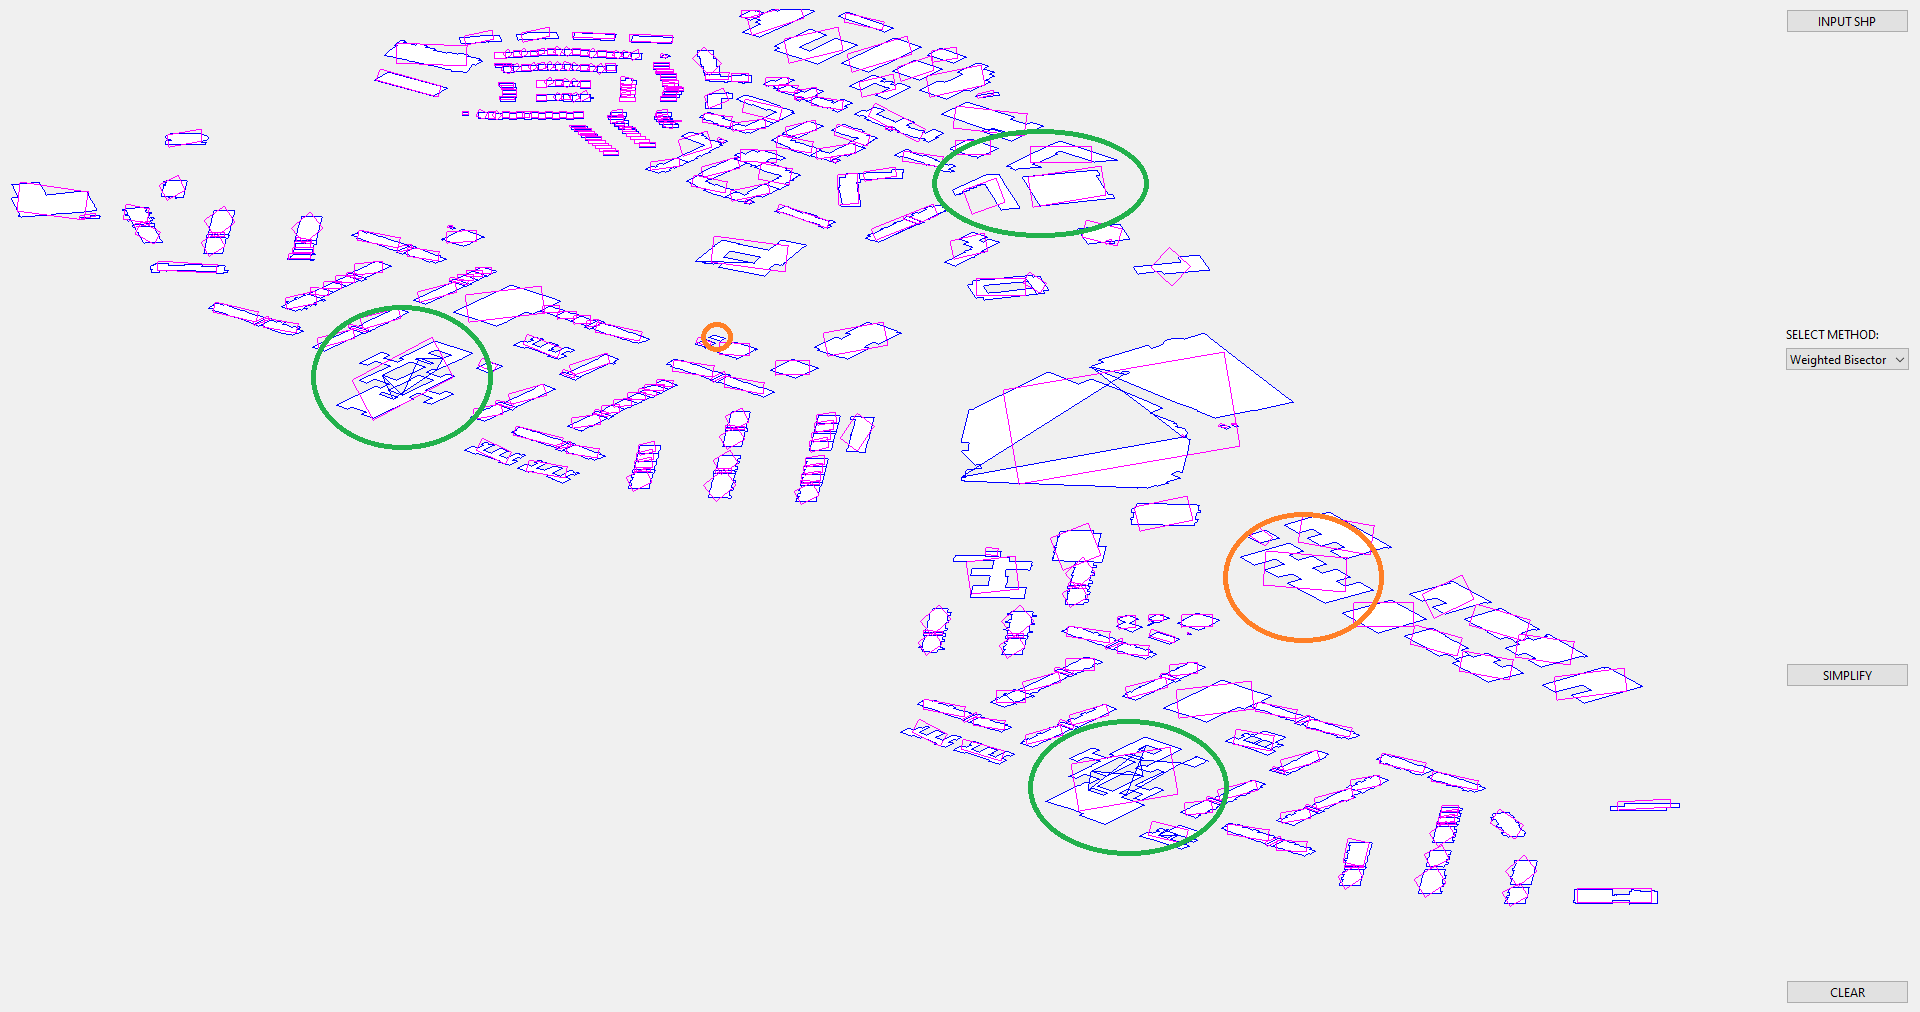
\includegraphics[width=14.65cm, height=7.5cm]{images/chodov_bi.png}
\caption{Generalizácia datasetu Chodov algoritmom \textit{Weighted Bisector}.}
\label{fig:obr21}
\end{figure}

Najlepšie výsledky pre tento dataset dosahuje \textit{Minimum Area Enclosing Rectangle}. Druhý najkvalitnejší je \textit{Weighted Bisector}, ktorý avšak jednu budovu negeneralizoval, pretože sa nepodarilo vypočítať jej uhlopriečky. Najhorším bol \textit{Longest Edge}, ktorý si neporadil s budovami podlhovastého tvaru, pri ktorých najdlhšia hrana celkom jednoznačne určuje orientáciu budovy. Problémom môže byť spracovanie súradníc vstupných dát, ktoré v tomto prípade rozdelí najdlhšie hrany do krátkych segmentov, čo zásadne ovplyvní tento algoritmus.

\newpage
\section{Dokumentácia}
Samotný program bol napísaný v jazyku Python 3.9 v SW PyCharm. Okrem externých modulov QT bol využitý aj modul \texttt{pyshp}, ktorý slúži na prečítanie SHP súboru. Program pozostáva z troch tried:
\begin{enumerate}
    \item  Trieda \texttt{MainForm}:\\
Predstavuje užívateľské rozhranie pre aplikáciu, obsahuje šesť metód:

Metódy \texttt{setupUi} a \texttt{retranslateUi} boli automaticky vygenerované prostredníctvom vývojového prostredia QT a prepisom QML do Pythonu.

Metóda \texttt{input} inicializuje vloženie vstupných dát do programu. Zisťuje šírku a výšku zobrazovacej plochy aplikácie z dôvodu nutného preškálovania súradníc vstupných dát do súradníc zobrazovacej plochy aplikácie. Hodnoty šírky a výšky sme redukovali o hodnotu 100, aby sme dosiahli offsetu od okrajov okna aplikácie. Následne sa tieto redukované hodnoty  predávajú metóde \texttt{setPath}.

Metóda \texttt{simplifyClick} sa týka tlačidla \textit{SIMPLIFY}, ktoré spúšťa proces generalizácie budov pomocou navoleného algoritmu v ComboBoxe. V metóde \texttt{simplifyClick} sa preto testuje, ktorý z algoritmov je aktuálne zvolený a má byť spustený (testuje sa hodnota aktuálneho indexu pomocou funkcie self.comboBox.currentIndex()). Index 0 odkazuje na algoritmus Minimum Area Enclosing Rectangle, index 1 na Wall Average, index 2 na Longest Edge a index 3 na Weighted Bisector. V metóde \texttt{simplifyClick} sú takisto inicializované pomocné premenné pre uloženie výsledkov.\newline
Následne sa iteruje cez každý element listu polygónov. V poslednom kroku prekresluje zobrazovaciu plochu.

Metóda \texttt{clearClick} sa týka tlačidla \textit{CLEAR}, ktoré zabezpečuje odstránenie akýchkoľvek útvarov na Widgete aplikácie.  

\newline
    \item Trieda \texttt{Draw}:\\
Je zodpovedná za grafickú stránku aplikácie a zobrazovacej plochy. Trieda obsahuje inicializátor a sedem metód:

\texttt{Inicializátor} má dva pozičné argumenty a inicializuje premenné pre túto triedu. Inicializovaný je prázdny list polygónov a takisto aj prázdny list výsledkov, do ktorého sa pri každej iterácií z metódy \texttt{analyze} ukladajú výsledky pre každý jeden polygón. \newline
Metóda \texttt{setPath} má dva argumenty a to šírku a výšku zobrazovacej plochy aplikácie. Do premennej ukladá cestu k SHP súboru, ktorý predstavuje vstupné dáta, ktorý užívateľ vyberie z pop-up okna. Na prečítanie SHP súboru sa využíva externý modul \texttt{pyshp}. \newline
V ďalšom kroku extrahuje súradnice zo SHP súboru a to tak, aby sa zachovala informácia, ktoré súradnice (vrcholy) tvoria ktorý polygón.\newline
Z dôvodu rozličného súradnicového systému vstupných dát a zobrazovacej plochy aplikácie vstupné dáta navyše preškálováva. V prvom rade je bod najbližší počiatku súradnicového systému zobrazovacej plochy presunutý do jeho počiatku. Následne sa vykoná normalizácia do intervalu $<0, 1>$ a hodnoty sú vynásobené šírkou a výškou zobrazovacej plochy. Navyše $Y$ súradnice preklápa cez osu $X$. \newline
Metóda vracia list polygónov.

Metódy \texttt{getPolygon} vracia list polygónov.

Metóda \texttt{setResult} pridáva do prázdneho listu výsledných generalizácií výsledky pre jednotlivé polygony budov. 

Metóda \texttt{paintEvent} má argument \texttt{QPaintEvent} z modulu \texttt{QtGui}. Dochádza tu ku začiatku vizualizácie na zobrazovacej ploche. Pomocou iterácií listu budov a listu výsledných generalizácií budov sa vykresľuje každý jeden polygon. Pre budovy ako aj pre ich generalizácie sa nastavuje rozličná farba.

    \item Trieda \texttt{Algorithms}:\\
Trieda obsahuje matematické metódy, pomocou ktorých sú realizované jednotlivé algoritmy analýzy, ktoré sú taktiež zapísané v tejto triede.

Metóda \texttt{getPointAndLinePosititon} má na vstupe tri argumenty, všetky predstavujú body v dátovom type \texttt{QPoint}. Slúži na určenie polohy analyzovaného bodu a priamky. \newline
V prvom kroku je definovaná prijateľná odchýlka \texttt{epsilon}, nasleduje výpočet zložiek dvoch vektorov a výpočet vektorového súčinu pomoocu determinantu a testovanie podmienok, do ktorých vstupuje hodnota determinantu a podľa ktorej sa určí pozícia bodu voči priamke. \newline
Metóda vracia hodnotu 1 ak je bod v ľavej polrovine, hodnotu 0 ak je bod v pravej polrovine, v prípade kolinearity vráti hodnotu -1.

Metóda \texttt{get2LinesAngle} má na vstupe štyri body, opäť všetky v dátovom type \texttt{QPoint}. Slúži na výpočet uhlu dvoch priamok. Opäť sú spočítané dva vektory, ich skalárny súčin a ich norma. \newline
Figuruje v nej podmienka, ktorá rieši singularitu analyzovaného bodu na vrchole polygónu, a to na základe nulovej hodnoty jednej z noriem vektorov. Metóda v tomto prípade vracia hodnotu 0.\newline
Druhá podmienka slúži na vyhnutie sa prípadu, kedy $\arccos$ uhlu dvoch priamok sa počíta z hodnoty, ktorá je väčšia ako 1. V takomto prípade metóda vracia výslednú hodnotu z $|\arccos(1)|$.\newline
Mimo spomenutých prípadov funkcia vracia hodnotu uhlu dvoch priamok v kladných hodnotách.

Metóda \texttt{jarvisScanCH} má na vstupe argument pol dátového typu \texttt{QPolygon} a argument length dátového typu \texttt{int}, ktorý predstavuje dĺžku aktuálne spracovaného polygonu. Je v nej implementovaný \textit{Jarvis Scan algoritmus}, ktorý je detailne popísaný v kapitole \ref{js}.
Metóda vracia konvexnú obálku vstupu (budova) v dátovom type \texttt{QPolygon}.

Metóda \texttt{grahamScanCH} má na vstupe rovnako ako predošlá metóda argument pol dátového typu \texttt{QPolygon} a rovnako ako predošlá metóda vracia konvexnú obálku vstupného polygonu v tvare \texttt{QPolygon}. Rozdiel je v implementovanom algoritme (namiesto Jarvis Scan je implementovaný Graham Scan, detailne popísaný v kapitole \ref{gs}.

Metóda \texttt{rotate} má na vstupe dva argumenty a to pol dátového typu \texttt{QPolygon} a angle dátového typu \texttt{float}. Pomocou tejto funkcie je vstupný polygon rotovaný o uhol angle. Výstupom je takto otočený polygon dátového typu \texttt{QPolygon}. 

Metóda \texttt{minMaxBox} má na vstupe pol dátového typu \texttt{QPolygon}. Funkcia vracia dva výstupy a to, obsah plochy výstupného polygonu Minimum Bounding Rectangle (typ \texttt{float}) a samotný \texttt{QPolygon}. Minimum Bounding Rectangle je popísaný v kapitole \ref{mbb}. 

Metóda \texttt{getArea} má na vstupe argument pol dátového typu \texttt{QPolygon}. Vo vnútri metódy je vypočítaný obsah nekonvexného vstupného polygonu. Tento obsah je vracaný v datovom type \texttt{float}.

Metóda \texttt{resizeRectangle} má na vstupe dva argumenty a to er a pol, oba dátového typu \texttt{QPolygon}. Er je v tejto úlohe chápaný ako Minimum Bounding Rectangle. Metóda vypočíta podiel obsahov oboch polygonov a prvý vstup (polygon er) zmenšuje/zväčšuje tak, aby jeho plocha bola rovnaká ako plocha polygonu pol. Takto modifikovaný polygon er je následne funkciou vracaný. 

Metóda \texttt{getLength} má na vstupe dva argumenty p1 a p2 rovnakého dátového typu \texttt{QPoint}. Metóda vracia dĺžku úsečky (v dátovom type \texttt{float}), ktorá je definovaná bodmi p1 a p2. 

Metóda \texttt{minAreaEnclosingRectangle} má na vstupe \texttt{QPolygon} pol, ďalej \texttt{int} ch a takisto lenght \texttt{int}. Integer ch predáva funkcii momentálny index druhého comboboxu a teda určuje, ktorý z algoritmov pre tvorbu konvexnej obálky bude aplikovaný. Argument lenght predáva funkcii dĺžku aktuálneho polygonu. V metóde je implementovaný algoritmus Minimum Area Enclosing Rectangle, popísaný v kapitole \ref{maer}. Vracia výslednú generalizáciu vstupného polygonu v tvare \texttt{QPolygon}. 

Metóda \texttt{wallAverage} má na vstupe \texttt{QPolygon} pol. V metóde je implementovaný algoritmus Wall Average, popísaný v kapitole \ref{wa}. Vracia výslednú generalizáciu vstupného polygonu v tvare \texttt{QPolygon}. 

Metóda \texttt{longestEdge} má na vstupe \texttt{QPolygon} pol. V metóde je implementovaný algoritmus Longest Edge, popísaný v kapitole \ref{le}. Vracia výslednú generalizáciu vstupného polygonu v tvare \texttt{QPolygon}. 

Metóda \texttt{weightedBisector} má na vstupe \texttt{QPolygon} pol. V metóde je implementovaný algoritmus Weighted Bisector, popísaný v kapitole \ref{bi}. Vracia výslednú generalizáciu vstupného polygonu v tvare \texttt{QPolygon}. 
 
\end{enumerate}

\newpage
\section{Záver}

Vytvorená aplikácia a program úspešne generalizuje budovy algoritmami \textit{Minimum Area Enclosing Rectangle}, \textit{Wall Average}, \textit{Longest Edge} a \textit{Weighted Bisector}. Takisto sú v nej implementované metódy \textit{Jarvis Scan} a \textit{Graham Scan} pre tvorbu konvexnej obálky, ktorá sa využíva v prvom menovanom algoritme.

Problémom aplikácie je správne prečítanie polygónovej vrstvy v prípade, ak obsahuje menší polygón v polygóne (napr. prípad enkláv), prípadne multipart polygóny. V takomto prípade vzniká úsečka medzi posledným bodom prvého polygónu a prvým bodom nasledujúceho polygónu enklávy. Táto úsečka negatívne ovplyvňuje výsledky.

\noindent Čo sa týka preškálovania vstupných dát kvôli ich vizualizácii, tak dochádza k jemnej deformácii tvaru územia a to kvôli roztiahnutiu dát v oboch smeroch do maximálneho možného intervalu.

\newpage
\setlength{\parindent}{0cm}
\section{Použité zdroje}
Prednášky z predmetu \textit{Algoritmy počítačové kartografie}.

BAYER, T. 2008: The importance of computational geometry for digital cartography. Geoinformatics FCE CTU, 3, s. 15–24.

DROPPOVÁ, V. 2011: The tools of automated generalization and building generalization in an ArcGIS environment. Slovak Journal of Civil Engineering, 19(1), s. 1–7.

DUCHENE, C. et al. 2003: Quantitative and qualitative description of building orientation.

LI, Z. et al. 2004: Automated building generalization based on urban morphology and Gestalt theory. International Journal of Geographical Information Science, 18, 5, s. 513-534.


\end{document}